% =============================================================================
%  SLR207 - Distributed Computing - Final Project Report
%  A from-scratch distributed MapReduce engine on the Télécom Paris cluster
%  Compile with:  pdflatex final_report.tex   (run twice for the ToC/refs)
% =============================================================================
\documentclass[11pt,a4paper]{article}

% ---- Encoding & fonts -------------------------------------------------------
\usepackage[utf8]{inputenc}
\usepackage[T1]{fontenc}
\usepackage{lmodern}
\usepackage[english]{babel}

% ---- Layout -----------------------------------------------------------------
\usepackage[margin=2.3cm]{geometry}
\usepackage{microtype}
\usepackage{parskip}
\usepackage{titlesec}
\usepackage{fancyhdr}
\usepackage{enumitem}
\setlist{itemsep=2pt,topsep=3pt}

% ---- Math, tables, graphics -------------------------------------------------
\usepackage{amsmath,amssymb}
\usepackage{graphicx}
\usepackage{booktabs}
\usepackage{tabularx}
\usepackage{multirow}
\usepackage{array}
\usepackage{caption}
\usepackage{float}
\usepackage{xcolor}

% ---- Diagrams ---------------------------------------------------------------
\usepackage{tikz}
\usetikzlibrary{arrows.meta,positioning,calc,shapes.geometric,backgrounds,fit}

% ---- Code listings ----------------------------------------------------------
\usepackage{listings}
\definecolor{codebg}{RGB}{246,248,250}
\definecolor{codekw}{RGB}{0,92,197}
\definecolor{codecm}{RGB}{106,115,125}
\definecolor{codestr}{RGB}{3,47,98}
\definecolor{accent}{RGB}{196,30,58}
\definecolor{accentblue}{RGB}{0,92,197}
\lstdefinestyle{mono}{
  basicstyle=\ttfamily\small,
  backgroundcolor=\color{codebg},
  keywordstyle=\color{codekw}\bfseries,
  commentstyle=\color{codecm}\itshape,
  stringstyle=\color{codestr},
  numberstyle=\tiny\color{codecm},
  breaklines=true,
  frame=single,
  framesep=4pt,
  rulecolor=\color{gray!30},
  showstringspaces=false,
  columns=fullflexible,
  keepspaces=true,
}
\lstset{style=mono}

% ---- Links ------------------------------------------------------------------
\usepackage[colorlinks=true,linkcolor=accentblue,urlcolor=accentblue,citecolor=accentblue]{hyperref}

% ---- Section styling --------------------------------------------------------
\titleformat{\section}{\Large\bfseries\color{accentblue}}{\thesection}{0.6em}{}
\titleformat{\subsection}{\large\bfseries}{\thesubsection}{0.6em}{}
\titlespacing*{\section}{0pt}{14pt}{6pt}

\pagestyle{fancy}
\fancyhf{}
\lhead{\small SLR207: Distributed MapReduce}
\rhead{\small Final Report}
\cfoot{\thepage}
\renewcommand{\headrulewidth}{0.4pt}

% ---- Helper macros ----------------------------------------------------------
\newcommand{\code}[1]{\texttt{\small #1}}

\begin{document}

% =============================================================================
%  TITLE PAGE
% =============================================================================
\begin{titlepage}
\centering
\vspace*{1.5cm}
{\Huge\bfseries A From-Scratch Distributed\\[0.3cm] MapReduce Engine\par}
\vspace{0.6cm}
{\Large\itshape Design, Fault Tolerance, Performance Analysis\\ and a Kafka Streams Comparison on Common Crawl\par}
\vspace{1.2cm}
\rule{0.8\textwidth}{0.8pt}\par
\vspace{0.5cm}
{\large \textbf{SLR207, Distributed Computing}\par}
{\large Télécom Paris\par}
\vspace{0.4cm}
{\large Final Written Report\par}
\rule{0.8\textwidth}{0.8pt}\par
\vspace{1.2cm}

{\large\textbf{Team}\par}
\vspace{0.3cm}
{\large Camil Daou \quad$\cdot$\quad Aymen Kabil \quad$\cdot$\quad Rémi Deloye \quad$\cdot$\quad Sébastien Riviere\par}
\vspace{1.4cm}

\begin{tabular}{rl}
\textbf{Course} & SLR207, Systèmes répartis / Distributed Computing\\[4pt]
\textbf{Subject} & Build a MapReduce engine on 100 lab machines\\[4pt]
\textbf{Data set} & Common Crawl (WET extracts)\\[4pt]
\textbf{Reference} & Dean \& Ghemawat, \emph{MapReduce}, OSDI'04\\[4pt]
\textbf{Deliverables} & engine, fault tolerance, 4 analyses, Kafka, this report\\
\end{tabular}

\vfill
{\large A self-built, dependency-free engine running over SSH on the\\
Télécom Paris cluster, no Hadoop, no HDFS, no root access.\par}
\vspace{1cm}
{\small \today}
\end{titlepage}

\tableofcontents
\newpage

% =============================================================================
\section{Introduction and project context}
% =============================================================================

This report documents, end to end, a distributed data-processing system built
from scratch over five lab sessions for the SLR207 course at Télécom Paris. The
goal was not to \emph{use} a big-data framework but to \emph{re-implement} the
core ideas of Google's MapReduce paper~\cite{mapreduce} on a real, shared,
constrained cluster (the school's 100+ lab machines), and to push it until it
broke, then make it robust.

\subsection{What was asked, session by session}

The project was specified incrementally across five guideline sessions. Every
single objective below is addressed in this report and implemented in the code.

\begin{table}[H]
\centering
\small
\renewcommand{\arraystretch}{1.25}
\begin{tabularx}{\textwidth}{@{}p{2.1cm}X@{}}
\toprule
\textbf{Session} & \textbf{Objectives}\\
\midrule
\textbf{Day 1} & Infrastructure: pick 100 live machines from the school API, deploy a TCP load-average server to all of them over SSH/NFS, query them in parallel from a client, write a clean-up script. (\S\ref{sec:cpuload})\\
\textbf{Day 2} & Study the MapReduce paper; design the Main/Workers protocol (KISS, no fault tolerance); space-time diagram; reducer key distribution $\mathrm{hash}(k)\bmod R$; understand NFS vs local disk. (\S\ref{sec:arch}, \S\ref{sec:protocol})\\
\textbf{Day 3} & Formalise the protocol on sequencediagram.org; solve bootstrap and remote-read; run word-frequency on real Common Crawl splits; (advanced) design fault tolerance and compare with Kafka Streams. (\S\ref{sec:protocol}, \S\ref{sec:cc})\\
\textbf{Day 4} & Per-phase timing and bottleneck detection; remove the internal NFS by reading Common Crawl directly from Amazon; test at micro / real / large scale; prove Amdahl's law empirically with a same-dataset speedup curve. (\S\ref{sec:perf}, \S\ref{sec:amdahl})\\
\textbf{Day 5} & Push to breaking point and add fault tolerance; deploy Kafka Streams without Docker/root; implement three analyses beyond word count; compare our system vs Hadoop vs Kafka Streams (batch vs stream); write this report and present. (\S\ref{sec:ft}, \S\ref{sec:jobs}, \S\ref{sec:kafka}, \S\ref{sec:compare})\\
\bottomrule
\end{tabularx}
\end{table}

\subsection{Design philosophy}

Three principles guided every decision:

\begin{itemize}
\item \textbf{KISS first, robustness second.} We built a deliberately simple,
correct V1 (no fault tolerance), measured it, and only then layered the
fault-tolerance protocol (V2) \emph{on top without changing the happy path}.
\item \textbf{No external dependencies, no privileges.} The engine is pure
Python standard library (NumPy is an optional accelerator). Everything runs as
an unprivileged user: no Hadoop, no HDFS, no Docker, no root, no ZooKeeper.
\item \textbf{Measure, never assume.} Every phase is timed and emitted as
machine-parsable log lines; the bottleneck and the Amdahl serial fraction are
\emph{measured}, and optimisations are justified by before/after numbers.
\end{itemize}

\subsection{Why Python}

We chose Python deliberately, not by default. It is one of the most widely used
languages in the world today --- and the default choice for data processing and
large-scale text/ML pipelines, exactly the domain a Common Crawl word-count
belongs to. Building the engine in Python let us ask a pointed
question: \emph{how far can we push an ``interpreted, GIL-bound, slow'' language
on a genuinely parallel workload before it becomes the bottleneck?} That framing
turned a potential weakness into one of the most interesting parts of the project. The
GIL forced our per-worker parallelism to be process-level (which maps cleanly
onto the distributed model), and the interpreter overhead made the MAP compute
the measured bottleneck --- which is precisely what drove the optimisation work
in \S\ref{sec:opt} and let us quantify the remaining gap with a C++ prototype
($\sim$1.7$\times$ compute). In short: Python maximised readability and
development speed, kept the standard-library-only constraint trivial to honour,
and gave us a concrete, honest baseline to optimise against and reason about.

\subsection{Repository map}

\begin{table}[H]
\centering
\small
\renewcommand{\arraystretch}{1.15}
\begin{tabularx}{\textwidth}{@{}lX@{}}
\toprule
\textbf{Path} & \textbf{Contents}\\
\midrule
\code{src/mapreduce/} & \code{master.py}, \code{worker.py}, \code{validate.py}, \code{download\_commoncrawl.py}\\
\code{src/server/}, \code{src/client/} & Day-1 CPU-load server and parallel client\\
\code{src/deploy/} & \code{deploy\_commoncrawl.sh}, \code{kill\_commoncrawl.sh}, \code{fault\_tolerance\_demo.sh}, \code{get\_machines.{sh,py}}\\
\code{src/kafka/} & \code{deploy\_kafka.sh}, \code{run\_wordcount.sh}, \code{commoncrawl\_source.sh}, \code{clean\_kafka.sh}\\
\code{src/benchmarks/} & \code{amdahl\_bench.py}, \code{plot\_amdahl.py}, \code{ssh\_parallelism\_sweep.py}, \code{find\_scratch.sh}, \code{local\_cluster.sh}\\
\code{tests/run\_all.py} & One-command single-machine harness (correctness + FT + Amdahl)\\
\code{doc/} & Guidelines, MapReduce paper, space-time SVGs, optimisation log\\
\code{report/} & This report and the generated Amdahl figures\\
\bottomrule
\end{tabularx}
\end{table}

\subsection{Contributions and collaboration}\label{sec:contrib}

The project was built by a team of four; the work split roughly along the
chronological phases of the project.

\begin{table}[H]
\centering
\small
\renewcommand{\arraystretch}{1.3}
\begin{tabularx}{\textwidth}{@{}lX@{}}
\toprule
\textbf{Member} & \textbf{Main responsibilities}\\
\midrule
\textbf{Rémi Deloye} & First part of the project: deployment scripts, and the
initial implementation and testing of the MapReduce engine (MAP/REDUCE cycle,
barrier, shuffle).\\
\textbf{Sébastien Rivière} & First part of the project (with Rémi): deployment
scripts, and implementing and testing the core MapReduce engine.\\
\textbf{Camil Daou} & Conception of the sequence diagrams; the \code{bench.py}
measurement library and the Amdahl study; bottleneck testing and the worker
optimisations (combine + bytes-regex + vectorised CRC32, parallel SSH shuffle,
on-demand ingestion).\\
\textbf{Aymen Kabil} & Deployment, the fault-tolerance layer (heartbeat/lease,
re-execution, straggler backups, atomic commit), the Kafka Streams comparison,
and integration of the remaining pieces of the system.\\
\bottomrule
\end{tabularx}
\end{table}

\noindent We collaborated through \textbf{GitHub}, using separate feature
branches per work-stream. We deliberately tried to work in a \emph{sequential}
manner --- merging one branch before starting the next --- to keep the shared
\code{master.py}/\code{worker.py} surface conflict-free. This held for most of
the project; near the end, with several optimisation, fault-tolerance and
benchmarking branches in flight at once, some merge conflicts became
unavoidable and were resolved by hand.

% =============================================================================
\section{Warm-up workflow: the CPU-load cluster (Day 1)}\label{sec:cpuload}
% =============================================================================

Before any MapReduce, Day 1 established the deployment muscle: getting code onto
100 machines and talking to them in parallel.

\textbf{Machine selection.} \code{get\_machines.sh} queries the school's
\code{tp.telecom-paris.fr/ajax.php} JSON endpoint (the same API the room-status
web page uses), filters for reachable hosts, and writes canonical names
(e.g.\ \code{tp-1a201-05.enst.fr}) to \code{runtime/machines.txt}.

\textbf{Server.} \code{src/server/server.py} is a minimal TCP server. On
each connection it reads \code{/proc/loadavg} and replies with the 1-, 5- and
15-minute load averages, then closes. It binds a \emph{dual-stack} IPv6 socket
(\code{IPV6\_V6ONLY=0}) with \code{SO\_REUSEADDR} for an instant restart,
and shuts down cleanly on \code{SIGTERM} / \code{SIGINT} to free the port.

\textbf{Deployment.} Because \code{\$HOME} is on NFS, a \emph{single} SCP copies
the server into the shared home; then one SSH per machine launches it. The
parallel client (\code{src/client/client.py}) fans out with a
\code{ThreadPoolExecutor}, collects every node's load, and prints per-node and
cluster-wide averages.

\textbf{Clean-up.} \code{kill\_cpuload.sh} kills the listener on the chosen port
and removes deployed files on every machine, essential for redeploying a new
version cleanly.

This workflow is the template the MapReduce deployment later reuses:
\emph{NFS for distribution, SSH for control, parallel fan-out, idempotent
clean-up}.

% =============================================================================
\section{System architecture}\label{sec:arch}
% =============================================================================

The engine is a classic \textbf{Main\,/\,Workers} (master/worker) MapReduce,
modelled directly on Figure~1 of Dean \& Ghemawat. The Main owns scheduling and
never touches the data; Workers do all I/O and computation.

\begin{figure}[H]
\centering
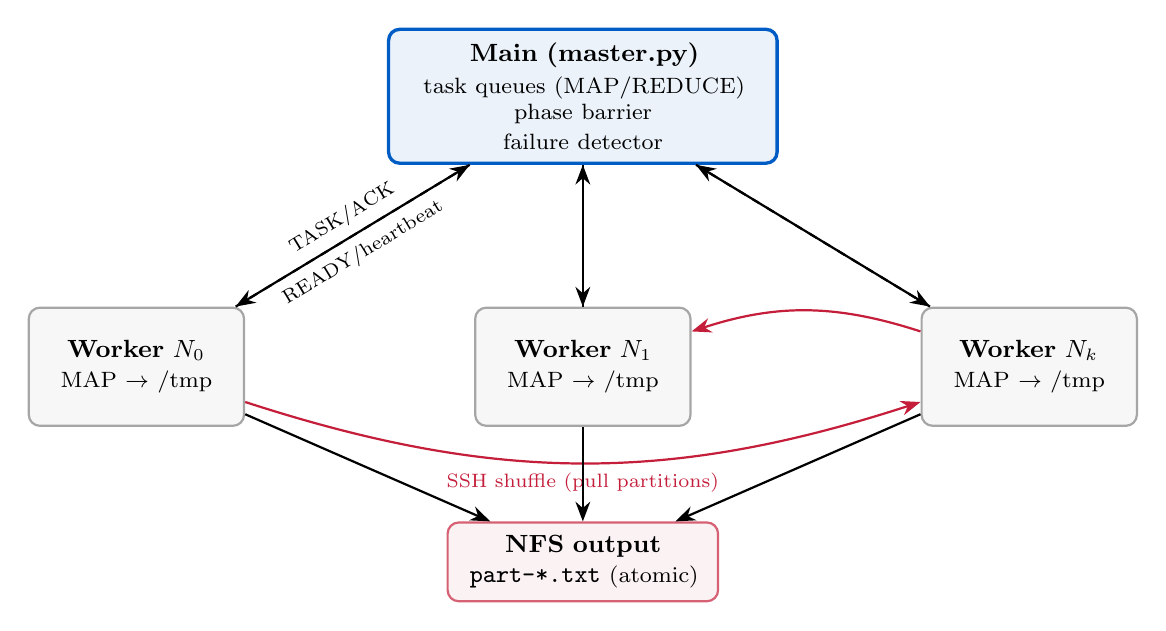
\begin{tikzpicture}[
  font=\small,
  node distance=8mm,
  main/.style={draw=accentblue,very thick,rounded corners,fill=accentblue!8,
               text width=4.7cm,align=center,minimum height=1.7cm},
  wk/.style={draw=gray!70,thick,rounded corners,fill=gray!6,
             text width=2.5cm,align=center,minimum height=1.5cm},
  nfs/.style={draw=accent!70,thick,rounded corners,fill=accent!6,
              text width=3.2cm,align=center,minimum height=1.0cm},
  arr/.style={-{Stealth[length=2.5mm]},thick},
]
% Main
\node[main] (main) {\textbf{Main (master.py)}\\[2pt]\footnotesize
  task queues (MAP/REDUCE)\\ phase barrier\\ failure detector};
% Workers
\node[wk,below left=18mm and 18mm of main] (w0) {\textbf{Worker $N_0$}\\\footnotesize MAP $\to$ /tmp};
\node[wk,below=18mm of main] (w1) {\textbf{Worker $N_1$}\\\footnotesize MAP $\to$ /tmp};
\node[wk,below right=18mm and 18mm of main] (w2) {\textbf{Worker $N_k$}\\\footnotesize MAP $\to$ /tmp};
% control arrows
\draw[arr] (main) -- (w0) node[midway,sloped,above,font=\scriptsize]{TASK/ACK};
\draw[arr] (main) -- (w1);
\draw[arr] (main) -- (w2);
\draw[arr,dashed] (w0) -- (main) node[midway,sloped,below,font=\scriptsize]{READY/heartbeat};
\draw[arr,dashed] (w1) -- (main);
\draw[arr,dashed] (w2) -- (main);
% shuffle
\draw[arr,accent] (w0) to[bend right=18] node[midway,below,font=\scriptsize,accent]{SSH shuffle (pull partitions)} (w2);
\draw[arr,accent] (w2) to[bend right=18] (w1);
% NFS output
\node[nfs,below=12mm of w1] (out) {\textbf{NFS output}\\\footnotesize \code{part-*.txt} (atomic)};
\draw[arr] (w0) -- (out);
\draw[arr] (w1) -- (out);
\draw[arr] (w2) -- (out);
\end{tikzpicture}
\caption{Main/Workers architecture. The Main routes \emph{metadata only}
(TCP, JSON lines). MAP intermediates stay on each worker's \emph{local} disk;
reducers pull partitions worker-to-worker over SSH; final output is committed
atomically to shared NFS.}
\label{fig:arch}
\end{figure}

\subsection{Components}

\begin{itemize}
\item \textbf{Main} (\code{master.py}) holds the MAP and REDUCE queues, drives
the \code{MAP$\to$REDUCE} barrier, tracks which worker holds which partition,
detects failures, and reassigns work. It binds a dual-stack IPv6 socket
\emph{before} loading tasks so early workers can connect and wait.
\item \textbf{Workers} (\code{worker.py}) register a unique identity, request
work in a pull loop, execute MAP or REDUCE, and report completion. A background
thread heartbeats the Main. Workers are identified by a \code{worker\_id} (not
just host), which lets several run on one machine, the basis of the
single-machine test mode.
\end{itemize}

\subsection{Storage model: NFS vs local disk}\label{sec:storage}

The school's \code{\$HOME} is on NFS; the paper insists MAP intermediates go to
\emph{local} disk. We honour both:

\begin{table}[H]
\centering
\small
\renewcommand{\arraystretch}{1.25}
\begin{tabularx}{\textwidth}{@{}llX@{}}
\toprule
\textbf{Data} & \textbf{Location} & \textbf{Rationale}\\
\midrule
Input splits (Common Crawl WET) & NFS, spill dir, \emph{or} in-memory stream & shared input, or bypass NFS entirely\\
MAP intermediate partitions & \textbf{local \code{/tmp}} (or \code{-{}-spill-dir}) & writing to NFS would hammer the shared server\\
REDUCE final output \code{part-*.txt} & NFS (shared) & collected in one place, written \emph{atomically}\\
Logs & local \code{/tmp/.../logs/<ts>} & per-run, off-NFS\\
\bottomrule
\end{tabularx}
\end{table}

Because \code{/tmp} can itself be a small RAM-backed \code{tmpfs} that saturates
under hundreds of concurrent MAP downloads, \code{src/benchmarks/find\_scratch.sh}
inspects \code{df}/\code{mount}, excludes NFS and pseudo-filesystems, and
recommends the largest \emph{local writable} partition; the worker's
\code{-{}-spill-dir} then redirects staging there.

% =============================================================================
\section{Network protocol design}\label{sec:protocol}
% =============================================================================

\subsection{Transport and message set}

Transport is \textbf{TCP}, one persistent connection per worker. Messages are
\textbf{newline-delimited JSON} (\code{\{...\}\textbackslash n}); both sides keep
a receive buffer to reassemble partial reads. The full message set:

\begin{table}[H]
\centering
\small
\renewcommand{\arraystretch}{1.2}
\begin{tabularx}{\textwidth}{@{}llX@{}}
\toprule
\textbf{Direction} & \textbf{Message} & \textbf{Purpose}\\
\midrule
W $\to$ M & \code{\{"status":"REGISTER","worker\_id":..,"host":..,"map\_dir":..\}} & announce identity + local map dir\\
W $\to$ M & \code{\{"status":"READY\_FOR\_TASK"\}} & request work\\
W $\to$ M & \code{\{"status":"TASK\_FINISHED"\}} & report completion\\
W $\to$ M & \code{\{"status":"HEARTBEAT"\}} & liveness ping (every 2\,s)\\
M $\to$ W & \code{\{"type":"MAP","split\_id":i,"n\_reducers":r,"job":J,"url":..\}} & assign a MAP\\
M $\to$ W & \code{\{"type":"REDUCE","reducer\_id":j,"map\_sources":[..],"job":J\}} & assign a REDUCE\\
M $\to$ W & \code{\{"type":"WAIT"\}} & nothing to do yet\\
M $\to$ W & \code{\{"status":"ACK"\}} & acknowledge a finish\\
\bottomrule
\end{tabularx}
\end{table}

A key design choice: \textbf{heartbeats are one-directional} (worker $\to$ Main).
This keeps the Main$\to$worker stream carrying only tasks and ACKs, so the
existing framing is untouched by fault tolerance.

\subsection{V1: the KISS protocol (no fault tolerance)}

The first version implements the bare cycle \code{MAP $\to$ barrier $\to$
SHUFFLE+REDUCE}. Each map worker writes one \code{partition\_j.txt} per reducer
to local disk. At reduce time, reducer $j$ fetches its partition file from
\emph{every} map worker via \code{ssh cat} and sums.

\begin{figure}[H]
\centering
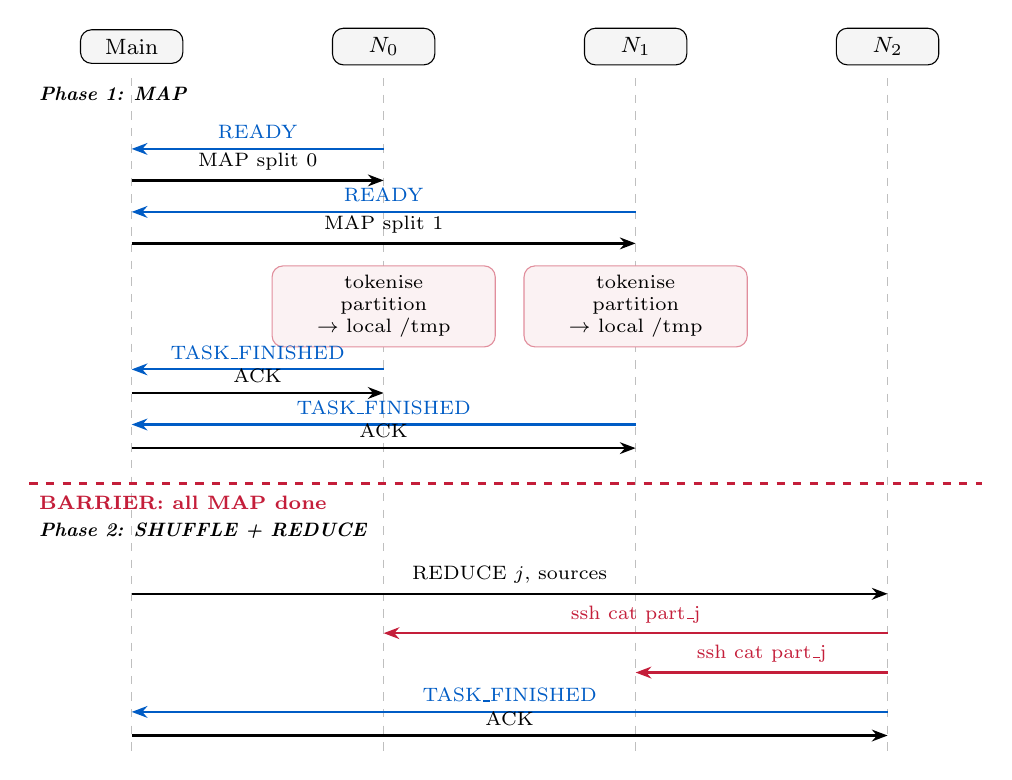
\begin{tikzpicture}[font=\footnotesize]
% lifelines
\def\xM{0} \def\xA{3.2} \def\xB{6.4} \def\xC{9.6}
\foreach \x/\name in {\xM/{Main}, \xA/{$N_0$}, \xB/{$N_1$}, \xC/{$N_2$}} {
  \node[draw,fill=gray!8,rounded corners,minimum width=1.3cm] at (\x,0) {\name};
  \draw[gray!50,dashed] (\x,-0.4) -- (\x,-8.95);
}
\tikzset{msg/.style={-{Stealth[length=2mm]},thick}}
\tikzset{ret/.style={-{Stealth[length=2mm]},thick,accentblue}}
% phase label
\node[accentblue,font=\bfseries] at (\xM,-0.9) {};
\node[anchor=west,font=\itshape\scriptsize] at (-1.3,-0.6) {\textbf{Phase 1: MAP}};
% READY / assign
\draw[ret] (\xA,-1.3) -- node[above,sloped,font=\scriptsize]{READY} (\xM,-1.3);
\draw[msg] (\xM,-1.7) -- node[above,sloped,font=\scriptsize]{MAP split 0} (\xA,-1.7);
\draw[ret] (\xB,-2.1) -- node[above,sloped,font=\scriptsize]{READY} (\xM,-2.1);
\draw[msg] (\xM,-2.5) -- node[above,sloped,font=\scriptsize]{MAP split 1} (\xB,-2.5);
% local write note
\node[draw=accent!50,fill=accent!6,rounded corners,font=\scriptsize,text width=2.6cm,align=center] at (\xA,-3.3) {tokenise\\ partition\\ $\to$ local /tmp};
\node[draw=accent!50,fill=accent!6,rounded corners,font=\scriptsize,text width=2.6cm,align=center] at (\xB,-3.3) {tokenise\\ partition\\ $\to$ local /tmp};
% finished
\draw[ret] (\xA,-4.1) -- node[above,sloped,font=\scriptsize]{TASK\_FINISHED} (\xM,-4.1);
\draw[msg] (\xM,-4.4) -- node[above,sloped,font=\scriptsize]{ACK} (\xA,-4.4);
\draw[ret] (\xB,-4.8) -- node[above,sloped,font=\scriptsize]{TASK\_FINISHED} (\xM,-4.8);
\draw[msg] (\xM,-5.1) -- node[above,sloped,font=\scriptsize]{ACK} (\xB,-5.1);
% barrier
\draw[very thick,accent,dashed] (-1.3,-5.55) -- (10.8,-5.55);
\node[anchor=west,accent,font=\bfseries\scriptsize] at (-1.3,-5.8) {BARRIER: all MAP done};
\node[anchor=west,font=\itshape\scriptsize] at (-1.3,-6.15) {\textbf{Phase 2: SHUFFLE + REDUCE}};
% reduce assign
\draw[msg] (\xM,-6.95) -- node[above,sloped,font=\scriptsize]{REDUCE $j$, sources} (\xC,-6.95);
% shuffle pulls
\draw[msg,accent] (\xC,-7.45) -- node[above,sloped,font=\scriptsize]{ssh cat part\_j} (\xA,-7.45);
\draw[msg,accent] (\xC,-7.95) -- node[above,sloped,font=\scriptsize]{ssh cat part\_j} (\xB,-7.95);
% reduce done
\draw[ret] (\xC,-8.45) -- node[above,sloped,font=\scriptsize]{TASK\_FINISHED} (\xM,-8.45);
\draw[msg] (\xM,-8.75) -- node[above,sloped,font=\scriptsize]{ACK} (\xC,-8.75);
\end{tikzpicture}
\caption{V1 (KISS) space-time diagram. The reducer for key $k$ is
$\mathrm{crc32}(k)\bmod R$. The Main only exchanges metadata; the actual
partition bytes flow worker-to-worker during SHUFFLE. (Full source rendered on
sequencediagram.org as \code{doc/map\_reduce/MapReduce.svg}.)}
\label{fig:v1}
\end{figure}

\subsection{Reducer key distribution}

Every analysis emits \code{(key, count)} pairs. The reducer responsible for a
key is chosen by hashing, exactly as in the paper:
\[
\text{reducer}(k) \;=\; \mathrm{crc32}(k) \bmod R .
\]
Because the same hash is used by every mapper, all occurrences of a key land in
the same reducer, so reduce outputs have disjoint key sets and never need
re-summing across reducers.

\subsection{Bootstrap}

A subtle ordering problem: workers may connect before the Main has finished
fetching \code{wet.paths.gz} and building its queues. The Main solves this by
\emph{binding and listening before loading tasks}; any worker that connects
early is parked on \code{WAIT} and retries until the queues are populated. This
gives a clean, race-free start-up.

% =============================================================================
\section{Common Crawl ingestion}\label{sec:cc}
% =============================================================================

Common Crawl publishes monthly crawls as WARC/WAT/WET files on
\code{data.commoncrawl.org}; we use the plain-text \textbf{WET} extracts. The
file list for a crawl is \code{crawl-data/<CRAWL\_ID>/wet.paths.gz}
(default crawl \code{CC-MAIN-2024-10}). It matters because Common Crawl is one of
the primary data sources used to train modern LLMs.

Three ingestion paths are implemented, from most to least NFS-dependent:

\begin{enumerate}
\item \textbf{Pre-download to NFS} (\code{download\_commoncrawl.py
-{}-missing-only}), idempotent; turns each WET \code{.gz} into a
\code{commoncrawl-XXXX.txt} split.
\item \textbf{On-demand download to the spill dir}, if the NFS split is absent
and the MAP task carries a \code{url}, the worker downloads it to local disk,
processes it, then deletes it.
\item \textbf{Direct read from Amazon into memory} (\code{-{}-direct-read}),
the worker streams and gunzips the \code{.wet.gz} straight from S3/HTTPS,
strips WARC/HTTP headers on the fly, and processes the bytes \emph{without ever
touching NFS or staging to disk}. This is the Day-4 mandate to ``retire the
internal NFS'' that saturates under massive concurrent reads.
\end{enumerate}

% =============================================================================
\section{The four analyses (pluggable jobs)}\label{sec:jobs}
% =============================================================================

All analyses share \emph{one} engine. The shuffle and reduce (sum by key, sort
descending) are identical; only the MAP keying differs, selected by
\code{-j/-{}-job} and implemented in a single function \code{\_map\_emit}. Every
job emits \code{bytes} keys so the downstream path is uniform.

\begin{table}[H]
\centering
\small
\renewcommand{\arraystretch}{1.3}
\begin{tabularx}{\textwidth}{@{}lll X@{}}
\toprule
\code{-j} & \textbf{Analysis} & \textbf{MAP key} & \textbf{Question answered}\\
\midrule
\code{wordcount} & word frequency & \code{word $\to$ 1} & which words are most frequent?\\
\code{lang} & language ranking & \code{stop-word hit $\to$ language} & which languages dominate the crawl?\\
\code{wordlen} & length distribution & \code{len(word) $\to$ 1} & what is the word-length histogram?\\
\code{bigram} & phrase popularity & \code{$w_1\;w_2 \to 1$} & which two-word phrases are most common?\\
\bottomrule
\end{tabularx}
\end{table}

\noindent\textbf{Methods.} \code{lang} matches each token against tiny,
high-frequency stop-word sets for en/fr/de/es/it; a token that is a stop-word in
exactly one language is a strong signal (tokens shared by several languages are
dropped to avoid bias). \code{wordlen} keys on \code{len(word)}; \code{bigram}
keys on consecutive word pairs $w_1\,w_2$.

\paragraph{What a bigram is, and ``function-word pairs dominate''.} A
\emph{bigram} is simply a pair of adjacent words in the text: sliding a
two-word window over ``\,the cat sat on\,'' yields the bigrams
\emph{the cat}, \emph{cat sat}, \emph{sat on}. Counting them tells us which
two-word phrases co-occur most often. The result is always led by
\emph{function words}, the grammatical ``glue'' of a language (articles,
prepositions, conjunctions, pronouns: \emph{the, of, in, to, and}), as opposed
to \emph{content words} (nouns, verbs) that carry topic meaning. Because a
handful of function words make up a huge share of all tokens, the pairs they
form (\emph{of the}, \emph{in the}, \emph{to the}) vastly outnumber any specific
content phrase. So ``function-word pairs dominate'' means the top of the bigram
ranking is grammatical glue, not topical phrases. It is a useful signal for spotting
templated/boilerplate text and a first step toward $n$-gram language modelling.

\subsection{Observed results on a real Common Crawl split}\label{sec:jobresults}

The tables below are \textbf{actual output} produced by the engine's own
\code{\_map\_emit} logic on a genuine Common Crawl split, the first WET file of
crawl \code{CC-MAIN-2024-10} (split
\code{...-00000.warc.wet.gz}), $\approx$62.9\,MB of
decompressed text, \textbf{6{,}622{,}954 tokens}. Each analysis is also checked
for internal consistency against the single-machine reference
(\S\ref{sec:validate}).

\paragraph{lang: language ranking.} Of the 611{,}007 single-language stop-word
hits, \textbf{English dominates with $\approx$79\%}, followed by the major
European languages in the expected order:

\begin{table}[H]
\centering
\small
\renewcommand{\arraystretch}{1.15}
\begin{tabular}{@{}lrrl@{}}
\toprule
rank & language & stop-word hits & share\\
\midrule
1 & \textbf{en} (English) & 483{,}085 & \textbf{79.06\%}\\
2 & fr (French)  & 65{,}300 & 10.69\%\\
3 & de (German)  & 33{,}684 & \phantom{0}5.51\%\\
4 & es (Spanish) & 19{,}048 & \phantom{0}3.12\%\\
5 & it (Italian) & \phantom{0}9{,}890 & \phantom{0}1.62\%\\
\bottomrule
\end{tabular}
\caption{\code{lang} observed result: English leads by a wide margin: exactly
Common Crawl's published language distribution, confirming the tokeniser sees
real multilingual web text.}
\end{table}

\paragraph{wordlen: word-length distribution.} The histogram is \emph{unimodal,
peaking at 2–4 characters} and decaying with a long tail (lengths run up to
161), the expected natural-language shape:

\begin{table}[H]
\centering
\small
\renewcommand{\arraystretch}{1.1}
\begin{tabular}{@{}rrrrrrrrr@{}}
\toprule
length & 2 & 4 & 3 & 5 & 1 & 6 & 7 & 8\\
\midrule
share & \textbf{16.0\%} & 15.5\% & 13.1\% & 12.3\% & 11.0\% & 8.6\% & 7.1\% & 5.9\%\\
\bottomrule
\end{tabular}
\caption{\code{wordlen} observed result: short tokens dominate; lengths 2–5
alone account for $\approx$57\% of all tokens. The very long ``words'' in the
161-bucket tail are non-text artefacts (URLs, hashes) in the WET extraction.}
\end{table}

\paragraph{wordcount: word frequency.} 435{,}471 distinct words; the head is the
usual English function words, mixed with multilingual tokens (\code{de}) and
some residual WET record-metadata tokens (\code{warc}, single digits):

\begin{table}[H]
\centering
\small
\renewcommand{\arraystretch}{1.1}
\begin{tabular}{@{}lrlrlrlr@{}}
\toprule
word & count & word & count & word & count & word & count\\
\midrule
\textbf{the} & 79{,}745 & a  & 76{,}287 & to & 58{,}487 & and & 49{,}884\\
of  & 48{,}187 & in & 42{,}100 & de & 47{,}992 & warc & 48{,}421\\
\bottomrule
\end{tabular}
\caption{\code{wordcount} observed result: \emph{the/a/to/and/of/in} top the
list as expected. \code{de} reflects French/Spanish content; \code{warc} and
bare digits are residual WET metadata (see the note below).}
\end{table}

\paragraph{bigram: phrase popularity.} 2{,}467{,}306 distinct pairs. Genuine
English collocations (\emph{of the}, \emph{refers to}) appear at the top
alongside WET record-metadata pairs:

\begin{table}[H]
\centering
\small
\renewcommand{\arraystretch}{1.1}
\begin{tabular}{@{}lrlr@{}}
\toprule
bigram & count & bigram & count\\
\midrule
\textbf{of the} & 9{,}984 & refers to & 6{,}948\\
urn uuid & 13{,}849 & warc record & \phantom{0}6{,}925\\
\bottomrule
\end{tabular}
\caption{\code{bigram} observed result: \emph{of the} / \emph{refers to} are
real high-frequency English phrases; \emph{urn uuid} / \emph{warc record} /
\emph{2024 02} are WET-header metadata pairs.}
\end{table}

\paragraph{A note on metadata noise.} The \code{warc}, \code{urn uuid} and
\code{warc record} entries are not English, they are tokens from the WET
\emph{record-metadata} headers (\code{WARC-Type}, \code{WARC-Record-ID:
<urn:uuid:...>}) that our deliberately lightweight header strip
(prefixes \code{WARC/}, \code{Content-}, \code{Metadata-}) leaves behind. This
is exactly the ``simple parsing $\Rightarrow$ minor metadata pollution''
trade-off flagged in the pain points (\S\ref{sec:pain}): \code{lang} and
\code{wordlen} are unaffected (they key on languages / lengths), while
\code{wordcount} and \code{bigram} surface it. A stricter \code{WARC-} prefix
filter removes it at the cost of a little extra parsing, a clean illustration of
the cost/precision trade-off in real-world data cleaning.

% =============================================================================
\section{The \code{bench.py} measurement library}\label{sec:bench}
% =============================================================================

Every optimisation in \S\ref{sec:opt} is justified by a before/after number, and
every one of those numbers had to be \emph{trustworthy}. That guarantee comes
from \code{src/benchmarks/bench.py}, a small ($\sim$380-line, zero-dependency)
statistical timing library we wrote before touching a single hot loop. It is the
instrument the rest of the performance story is measured with, so it earns its
own section.

\subsection{Why we built it (and why not a bare chronometer)}

The naïve way to time code is a single \code{time.time()} delta. We rejected it
for three concrete reasons:
\begin{itemize}
\item \textbf{\code{time.time()} is not monotonic.} It follows the wall clock, so
an NTP correction or a DST jump mid-measurement silently corrupts the delta.
\code{bench.py} uses \code{time.perf\_counter\_ns()} --- a monotonic,
nanosecond-resolution clock that never runs backwards.
\item \textbf{One number is not a measurement.} A phase that runs many times (one
TCP query per node, one MAP per split) has a \emph{distribution}, not a value. A
single sample cannot tell a stable 30\,ms from a 30\,ms mean hiding a 200\,ms
tail. We needed variance, percentiles, and a stability signal.
\item \textbf{``Optimise the bottleneck'' requires knowing the bottleneck.}
Guessing which phase dominates is how projects waste effort tuning code that is
$2\%$ of the wall. We wanted the tool itself to \emph{attribute} time to phases
and categories and name the culprit.
\end{itemize}
In short, we wanted the guarantees a tool like \emph{Google Benchmark} gives, but
embedded in the project and aware of our own phase taxonomy.

\subsection{How it works}

The library is built around a \code{Registry} that stores every timed span as a
\emph{sample} keyed by a label, and exposes three ways to feed it plus a
reporting/export back end.

\begin{itemize}
\item \textbf{\code{phase(label, category)}} --- a context manager that times an
arbitrary block and records one sample.
\item \textbf{\code{@timed(...)}} --- a decorator that records one sample per call
of a function.
\item \textbf{\code{benchmark(label, fn, min\_time, warmup)}} --- the
Google-Benchmark micro-benchmark loop: it runs \code{warmup} discarded
iterations (to page in code and warm caches), then calls \code{fn} repeatedly,
recording \emph{every} iteration as a sample, until a wall budget of
\code{min\_time} seconds has accumulated. This auto-scales the iteration count so
a 1\,µs kernel and a 1\,s kernel are both measured to the same statistical
confidence.
\end{itemize}

Each sample carries a \textbf{category} --- \code{io}, \code{network},
\code{compute}, \code{sync}, \code{deploy}, \code{cleanup} --- which is exactly
the Day-4 breakdown the brief asks for. A representative use, comparing the MAP
tokeniser candidates that became Optimisation~1:

\begin{lstlisting}[language=python]
import bench

raw = open("commoncrawl-0000.txt", "rb").read()

# auto-scaled micro-benchmarks: warm up, then loop until 0.5s of samples
bench.benchmark("map:baseline",      lambda: baseline_split_isalnum(raw))
bench.benchmark("map:bytes-regex",   lambda: _WORD_RE.findall(raw))
bench.benchmark("map:combine+crc32", lambda: map_emit(raw, n_reducers))

bench.report(title="MAP tokeniser candidates")   # ranks phases, names bottleneck
bench.save_json("map_bench.json")                 # raw samples for plotting
\end{lstlisting}

From the collected samples, \code{stats()} computes a full \code{Stats} record
per label:

\begin{table}[H]
\centering
\small
\renewcommand{\arraystretch}{1.2}
\begin{tabularx}{\textwidth}{@{}lX@{}}
\toprule
\textbf{Metric} & \textbf{Why it is reported}\\
\midrule
count, total & how many samples, and their summed time (drives the \% ranking)\\
mean, median & central tendency; median resists outliers the mean does not\\
p90, p95 & tail latency --- what a ``slow'' occurrence actually costs\\
stdev, min, max & spread of the distribution\\
\textbf{CV} $=\sigma/\mu$ & dimensionless \emph{stability}: the library flags any
phase with $\ge 5$ samples and $\mathrm{CV}>0.5$ as \textbf{high variance}\\
\bottomrule
\end{tabularx}
\caption{The per-phase statistics \code{bench.py} reports. Percentiles use linear
interpolation over the sorted samples.}
\end{table}

\code{report()} then sorts phases by total time, prints a per-category roll-up,
and explicitly names the \textbf{bottleneck phase} and \textbf{bottleneck
category} --- so the tool answers ``what should I optimise?'' directly rather than
leaving it to eyeballing. \code{save\_json()} dumps the raw per-sample series
(clock, unit, samples, and the derived stats), which is the format the plotting
scripts (\S\ref{sec:perf}) consume.

\subsection{How it was used, and how it helped}

\code{bench.py} was the decision procedure behind the optimisation work, not an
afterthought:
\begin{itemize}
\item \textbf{It located the bottleneck first.} Before optimising, the category
roll-up showed \code{compute} at \textbf{>85\%} of worker time, proving the MAP
tokeniser --- not I/O or network --- was the thing to attack. That single result
is what justified spending effort on the bytes-regex + combine + vectorised CRC32
of Optimisation~1 (\S\ref{sec:opt}) instead of, say, the shuffle.
\item \textbf{It compared candidates fairly.} The auto-scaling
\code{benchmark()} loop let us race \code{split()+isalnum()} against the
bytes-regex and the combine path on the \emph{same} input to the same time
budget, so the $1.52\times$ compute speed-up is a measured ratio of stable means,
not a lucky single run.
\item \textbf{It told us when a number was noise.} The CV / high-variance flag
kept us honest: network- and shuffle-category phases that showed
$\mathrm{CV}>0.5$ were reported as unstable, which is precisely why the shuffle
tuning was validated with a dedicated sweep
(\code{ssh\_parallelism\_sweep.py}) rather than a single timing.
\item \textbf{It produced the evidence.} The JSON export is the raw material
behind the tables and figures in \S\ref{sec:opt} and the Amdahl study
(\S\ref{sec:amdahl}); the same sample-based, per-phase, per-category methodology
is mirrored by the distributed \code{WORKER\_TIMING} instrumentation
(\S\ref{sec:perf}) that measures the real cluster.
\end{itemize}
The payoff is a project where ``we optimised X and it got faster'' is never a
claim of faith: every such statement traces back to a distribution of samples
collected by this library.

% =============================================================================
\section{Optimisations}\label{sec:opt}
% =============================================================================

We started from a deliberately naïve worker, measured it, and optimised the
\emph{proven} bottleneck --- never a guessed one. Every number below comes from
the raw per-phase benchmark logs
(\code{amdahl\_results\_\{python,opt1,opt2,cpp\}.json}) captured on the
\emph{same} 32-split, 8-reducer workload, so all four worker builds are directly
comparable row-by-row. The methodology (warm-up, fixed-budget timing, the
speed-up and Karp--Flatt derivations) is detailed in \S\ref{sec:amdahl}; here we
report the outcomes.

\subsection{Baseline (naïve worker)}

\code{line.split()} + \code{isalnum()} tokenisation; \code{crc32} called once
\emph{per word occurrence}; UTF-8 text I/O; one \code{word\textbackslash t1}
line per occurrence; \emph{sequential} SSH shuffle. Profiling showed
\code{t\_compute} is \textbf{>85\%} of worker time, the MAP loop is the
bottleneck, not I/O or network.

\subsection{Optimisation 1: combine + bytes-regex + vectorised CRC32}

\begin{itemize}
\item \textbf{Bytes-regex tokeniser} \code{re.compile(rb'[A-Za-z0-9]+')}: a
single pass over raw bytes, no UTF-8 decode, no per-line loop.
\item \textbf{Combine before partition}: aggregate \emph{all} occurrences into
one dict first, so \code{crc32} is called once per \emph{unique} key, not per
occurrence.
\item \textbf{Vectorised CRC32}: \code{np.frompyfunc(zlib.crc32,1,1)} over the
array of unique keys (with a pure-Python fallback when NumPy is absent).
\item \textbf{Batched \code{writelines}} instead of one write per word.
\end{itemize}

The three ideas are visible in \code{src/mapreduce/worker.py} (\code{\_map\_emit}
and \code{\_execute\_map}):

\begin{lstlisting}[language=python]
# 1. tokenise raw BYTES in one pass: no UTF-8 decode, no per-line loop
_WORD_RE = re.compile(rb'[A-Za-z0-9]+')
tokens   = _WORD_RE.findall(raw_data)

# 2. COMBINE: fold every occurrence into a dict -> one entry per UNIQUE key
counts = {}
for tok in tokens:
    k = tok.lower()
    counts[k] = counts.get(k, 0) + 1

# 3. vectorised CRC32 over the UNIQUE keys only (pure-Python fallback if no NumPy)
_crc32_vec = np.frompyfunc(zlib.crc32, 1, 1)
rids = _crc32_vec(keys).astype(np.int64) % n_reducers
\end{lstlisting}

\begin{table}[H]
\centering
\small
\renewcommand{\arraystretch}{1.2}
\begin{tabular}{@{}rrrrrr@{}}
\toprule
$N$ & base $t_{\text{total}}$ & opt1 $t_{\text{total}}$ & base compute & opt1 compute & speed-up (total)\\
\midrule
1  & 275.4 & 174.4 & 234.9 & 156.2 & \textbf{1.58$\times$}\\
2  & 148.2 &  99.3 & 233.8 & 154.6 & 1.49$\times$\\
4  &  92.8 &  68.7 & 235.4 & 154.4 & 1.35$\times$\\
8  &  53.5 &  40.6 & 235.7 & 154.8 & 1.32$\times$\\
16 &  55.4 &  45.2 & 235.6 & 154.6 & 1.23$\times$\\
32 &  61.2 &  47.7 & 235.9 & 154.8 & 1.28$\times$\\
\bottomrule
\end{tabular}
\caption{Baseline vs Optimisation 1 (seconds, 32 splits). Compute is a
consistent \textbf{1.52$\times$} faster. As a free bonus, the combine phase
shrinks each partition to one line per \emph{unique} word, cutting
\code{t\_shuffle} \textbf{4–5$\times$}.}
\end{table}

\subsection{Optimisation 2: parallel SSH shuffle with connection multiplexing}

The reducer fetches all partitions concurrently with a
\code{ThreadPoolExecutor}, turning shuffle wall-time from $O(N\cdot\text{latency})$
into $\approx O(\text{latency})$. To avoid tripping the cluster's
\code{fail2ban}/IDS with a burst of SSH connections, we enable
\code{ControlMaster=auto} multiplexing: the first SSH to a host opens one real
TCP connection and all subsequent fetches (even from other reducers on the same
machine) reuse it. A sweep (\code{ssh\_parallelism\_sweep.py}) showed shuffle
wall-time \emph{floors} at \code{max\_ssh}~$\approx$~6–8 for $N\le32$, so the
default is \code{min(n\_workers, 8)}.

The shuffle loop in \code{worker.py} (\code{\_execute\_reduce}):

\begin{lstlisting}[language=python]
# one real TCP connection per host, reused by every later fetch
ssh_opts = ("-o ControlMaster=auto "
            "-o ControlPath=/tmp/ssh-ctrl-%h-{port} -o ControlPersist=120s")

# fetch all partitions concurrently: wall-time ~ slowest single fetch
with ThreadPoolExecutor(max_workers=min(len(sources), 8)) as ex:
    futures = {ex.submit(fetch_partition, s): s for s in sources}  # ssh host 'cat partition_j'
    for fut in as_completed(futures):
        all_raw_lines.extend(fut.result()[1])
\end{lstlisting}

The direct effect is visible in the \code{t\_shuffle} column: the sequential
reducer paid a shuffle cost that \emph{grew} with $N$ (more mappers to pull from,
one at a time), whereas the parallel reducer's shuffle wall-time stays flat and
small because it equals the \emph{slowest single} fetch, not their sum.

\begin{table}[H]
\centering
\small
\renewcommand{\arraystretch}{1.2}
\begin{tabular}{@{}rrrrr@{}}
\toprule
$N$ & opt1 $t_{\text{shuffle}}$ & opt2 $t_{\text{shuffle}}$ & opt1 $t_{\text{total}}$ & opt2 $t_{\text{total}}$\\
\midrule
1  &  4.8 & 1.2 & 174.4 & 127.7\\
2  &  9.4 & 1.4 &  99.3 &  64.6\\
4  & 16.8 & 2.1 &  68.7 &  39.9\\
8  & 27.6 & 3.9 &  40.6 &  35.1\\
16 & 28.2 & 2.8 &  45.2 &  39.4\\
32 & 26.9 & 4.8 &  47.7 &  36.4\\
\bottomrule
\end{tabular}
\caption{Optimisation 1 vs Optimisation 2 (seconds, 32 splits). The
\code{t\_shuffle} column isolates the parallel-SSH change: a \textbf{5--8$\times$}
reduction that no longer scales with the number of mappers. \code{t\_total} also
improves because Opt2 is measured on the fully-tuned Python worker.}
\end{table}

\subsection{What the optimisations moved --- and what they did not}
\label{sec:opt-scaling}

A subtle but important point for the Amdahl discussion (\S\ref{sec:amdahl}): the
optimisations \textbf{clearly lower the absolute wall-clock time}, but they
\textbf{do not improve --- and in fact reduce --- the parallel speed-up ratio}.
The two are not contradictory; they are the expected consequence of Amdahl's law.

\begin{table}[H]
\centering
\small
\renewcommand{\arraystretch}{1.2}
\begin{tabular}{@{}lrrrr@{}}
\toprule
worker build & $t_{\text{total}}(1)$ & best $t_{\text{total}}$ & peak speed-up & Karp--Flatt $e$ ($N{=}8$)\\
\midrule
Baseline (na\"ive)      & 275.4 & 53.5 (N=8)  & 5.15$\times$ & 0.079\\
Opt1 (compute)          & 174.4 & 40.6 (N=8)  & 4.30$\times$ & 0.123\\
Opt2 (+parallel shuffle)& 127.7 & 35.1 (N=8)  & 3.64$\times$ & 0.172\\
C++ worker (prototype)  & 132.5 & 35.5 (N=16) & 3.73$\times$ & 0.180\\
\bottomrule
\end{tabular}
\caption{Scalability summary across worker builds (32 splits). The absolute wall
drops \textbf{53.5$\to$40.6$\to$35.1\,s}, yet peak speed-up \emph{falls}
(5.15$\to$3.64$\times$) and the Karp--Flatt serial fraction \emph{rises}
(0.079$\to$0.172).}
\end{table}

\textbf{Why the wall moves but the speed-up shrinks.} The Karp--Flatt metric
$e = \left(\tfrac{1}{S_p}-\tfrac{1}{p}\right)\big/\left(1-\tfrac{1}{p}\right)$
estimates the \emph{experimentally serial fraction}. Each optimisation attacks
the \emph{parallel} part (per-split MAP compute), so it shrinks the numerator of
the parallel work while the fixed serial/overhead cost (job setup, the final
merge, and especially shuffle/NFS traffic) stays roughly constant. By Amdahl,
making the parallel part cheaper \emph{raises} the serial \emph{fraction} of what
remains --- hence a smaller speed-up even though every configuration finishes
sooner in absolute terms. This is the correct, healthy outcome: we were paid in
latency, not in a better slope.

\textbf{The true ceiling is NFS-read contention, not a serial code path.} All
builds reach their floor at $N{\approx}8$ and then \emph{regress} (e.g.\ Opt1:
40.6\,s at $N{=}8$ but 47.7\,s at $N{=}32$). The cause is visible in the phase
logs: \code{t\_io\_read} grows with $N$ (Opt1 rises from 3.4\,s at $N{=}1$ to
\textbf{69\,s} at $N{=}32$) because every worker reads its split from the shared
NFS home at once. This is an \emph{overhead} wall, not a fixed serial fraction,
and it is precisely what the on-demand Common Crawl ingestion
(\S\ref{sec:cc}) removes by having each worker pull its own split directly from
Amazon into local \code{/tmp}.

\subsection{Optimisation 3: on-demand ingestion --- and its superlinear scaling}
\label{sec:opt-ondemand}

The mechanism is described in \S\ref{sec:cc} (path~2): when the master ships a
\code{url} with each MAP task, the worker downloads its split to local
\code{/tmp}, processes it, and deletes it --- the shared NFS home is never
touched on the read path. We benchmarked it on the real 32-split
\code{CC-MAIN-2024-10} crawl to confirm it removes the contention wall above,
and it produced the most interesting curve in the whole study: a
\textbf{superlinear} speed-up ($S(N)>N$).

\begin{table}[H]
\centering
\small
\renewcommand{\arraystretch}{1.2}
\begin{tabular}{@{}rrrrrr@{}}
\toprule
$N$ & $t_{\text{total}}$ & speed-up & ideal & $t_{\text{dl,max}}$ & $t_{\text{io\_read}}$\\
\midrule
1 & 1646.6 & 1.00$\times$          & 1$\times$ & 172.2 & 16.1\\
2 &  603.7 & \textbf{2.73$\times$} & 2$\times$ &   9.0 &  2.2\\
4 &  307.8 & \textbf{5.35$\times$} & 4$\times$ &   8.6 &  1.5\\
8 &  199.1 & \textbf{8.27$\times$} & 8$\times$ &  11.6 &  1.6\\
\bottomrule
\end{tabular}
\caption{On-demand ingestion (seconds, 32 splits, \code{CC-MAIN-2024-10}).
Speed-up \emph{exceeds} ideal-linear at every point. \code{t\_dl,max} is the
longest single split download and \code{t\_io\_read} the local-disk read time.}
\label{tab:ondemand}
\end{table}

\begin{figure}[H]
\centering
\includegraphics[width=\textwidth]{amdahl_ondemand.png}
\caption{On-demand ingestion. Left: the measured speed-up sits \emph{above} the
ideal-linear diagonal (the shaded superlinear region), reaching $8.27\times$ at
$N{=}8$. Right: the mechanism --- the longest single split download
(\code{t\_dl,max}) collapses from 172\,s at $N{=}1$ (one node, one throttled S3
link) to $\approx$9\,s the instant a second node shares the load, so adding
workers relieves a per-node bottleneck at the same time as it divides the work.}
\label{fig:ondemand}
\end{figure}

\textbf{What it fixes.} The read path no longer goes through NFS, so
\code{t\_io\_read} stays flat at $\approx$1.5\,s for $N\ge2$ instead of climbing
to 69\,s (\S\ref{sec:opt-scaling}); the $\sim$5\,GB NFS quota and the separate
pre-staging step both disappear, and each node only ever fetches the handful of
splits it will actually process.

\textbf{Why the curve goes superlinear (the advantage).} Amdahl assumes the work
and the machine are fixed, so $S(N)\le N$. Here the \emph{per-node} resource
budget changes with $N$. At $N{=}1$ a single node must pull all 32 splits over
\emph{one} network link and one disk: the longest single download alone is
\textbf{172\,s} (one IP hammering S3 gets throttled), and the serialised
downloads dominate the 1647\,s baseline. Add nodes and the aggregate download
bandwidth and the number of independent local disks both grow with $N$, so
\code{t\_dl,max} collapses from 172\,s to $\approx$9\,s the moment a second
machine joins. The parallelisable work is therefore divided by $N$ \emph{while}
a per-node bottleneck is simultaneously relieved --- the two effects compound and
push $S(N)$ above the diagonal.

\textbf{The setbacks.} The same physics that makes the curve pretty makes it
dishonest as an efficiency metric, and expensive at small $N$:
\begin{itemize}
\item \textbf{A pathological serial baseline.} The superlinear number is inflated
by a crippled $N{=}1$ (1647\,s here vs $\approx$61\,s for the pre-staged path in
\S\ref{sec:opt-scaling}). It measures \emph{escape from a resource bottleneck},
not genuine compute parallelism, so it should not be read as ``better than
perfect scaling''.
\item \textbf{Amdahl no longer bounds it.} Because per-node bandwidth and cache
change with $N$, the fixed-work model does not apply; the curve cannot be
extrapolated with a single serial fraction $f$ the way the pre-staged sweeps can
(\S\ref{sec:amdahl}).
\item \textbf{External dependency and non-reproducibility.} Wall-time is now
hostage to S3 bandwidth and throttling; \code{t\_download} varies run-to-run and
the experiment is no longer self-contained.
\item \textbf{Re-download on failure.} A re-executed MAP (\S\ref{sec:ft}) must
re-fetch its split from the internet, since nothing is cached on NFS.
\end{itemize}
The takeaway: on-demand ingestion is the right choice at scale (it removes the
NFS wall and lets download I/O parallelise across nodes), but its superlinear
speed-up is a symptom of a resource-starved baseline, not a free lunch.

\textbf{Future ideas} (logged, not all benchmarked): gzip partitions before
transfer, \emph{push} partitions after MAP instead of pulling, replace SSH with
raw TCP, and finishing the C++ worker (the \code{cpp-worker} prototype already
gives $\sim$1.7$\times$ compute over the tuned Python worker, confirming the
remaining cost is the interpreter, not the algorithm).

% =============================================================================
\section{Performance instrumentation}\label{sec:perf}
% =============================================================================

Every phase of the lifecycle is timed and emitted as a structured, grep-able log
line, satisfying the Day-4 requirement to time deploy, clean, I/O, sync/wait,
network, and compute separately.

\begin{itemize}
\item \textbf{Main} emits \code{TIMING: \{"t\_total","t\_map","t\_reduce"\}}.
\item \textbf{Workers} emit one \code{WORKER\_TIMING} line per task:
\code{t\_download, t\_clean, t\_io\_read, t\_compute} for MAP and
\code{t\_shuffle, t\_compute, t\_io\_write} for REDUCE.
\end{itemize}

Two harnesses parse these lines into \code{runtime/amdahl\_results.json}, which
\code{plot\_amdahl.py} renders:

\begin{itemize}
\item \code{tests/run\_all.py}, a \textbf{single-machine} harness (several
worker processes on \code{localhost}, local-disk shuffle) that reproduces the
\emph{entire} pipeline (correctness, fault tolerance, and the Amdahl sweep)
with one command and no cluster.
\item \code{src/benchmarks/amdahl\_bench.py}, the \textbf{multi-node cluster}
sweep ($N=1,2,4,8,16,\dots$ real machines over SSH), same methodology, larger $N$.
\end{itemize}

The \textbf{measured bottleneck} is unambiguous: on the baseline worker
\code{t\_compute} is over 85\% of worker time; on the cluster the per-worker MAP
compute dominates and the REDUCE/shuffle is comparatively small
(Fig.~\ref{fig:cluster}, right panel).

% =============================================================================
\section{Amdahl's law: empirical validation}\label{sec:amdahl}
% =============================================================================

\subsection{Method and the correctness rule}

The reference point is $N=1\Rightarrow S=1$, and speedup is
$S(N) = t_{\text{total}}(1) / t_{\text{total}}(N)$. The
\emph{same dataset is reused at every point}: changing the data between points
would invalidate the comparison, as the brief stresses. We only interpolate
under the linear-scaling hypothesis on a \emph{single} machine; with $\ge 2$
nodes we \emph{measure}. Amdahl's law states
\[
S(N) \;=\; \frac{1}{f + \dfrac{1-f}{N}},
\qquad \lim_{N\to\infty} S(N) = \frac{1}{f},
\]
where $f$ is the incompressible serial fraction.

\subsection{Cluster results (real machines over SSH)}

The headline result is the multi-node sweep on 16 real Common Crawl splits
(8 reducers), the same dataset at every $N$:

\begin{table}[H]
\centering
\small
\renewcommand{\arraystretch}{1.2}
\begin{tabular}{@{}rrrrr@{}}
\toprule
$N$ & $t_{\text{total}}$ (s) & $t_{\text{map}}$ (s) & $t_{\text{reduce}}$ (s) & speedup\\
\midrule
1  & 521.66 & 490.55 & 31.11 & 1.00$\times$\\
2  & 262.80 & 245.26 & 17.54 & 1.99$\times$\\
4  & 137.15 & 126.89 & 10.26 & 3.80$\times$\\
8  &  84.60 &  77.69 &  6.91 & 6.17$\times$\\
16 &  67.37 &  60.99 &  6.38 & \textbf{7.74$\times$}\\
\bottomrule
\end{tabular}
\caption{Cluster Amdahl sweep (16 splits, 8 reducers, same dataset throughout).}
\label{tab:cluster}
\end{table}

\begin{figure}[H]
\centering
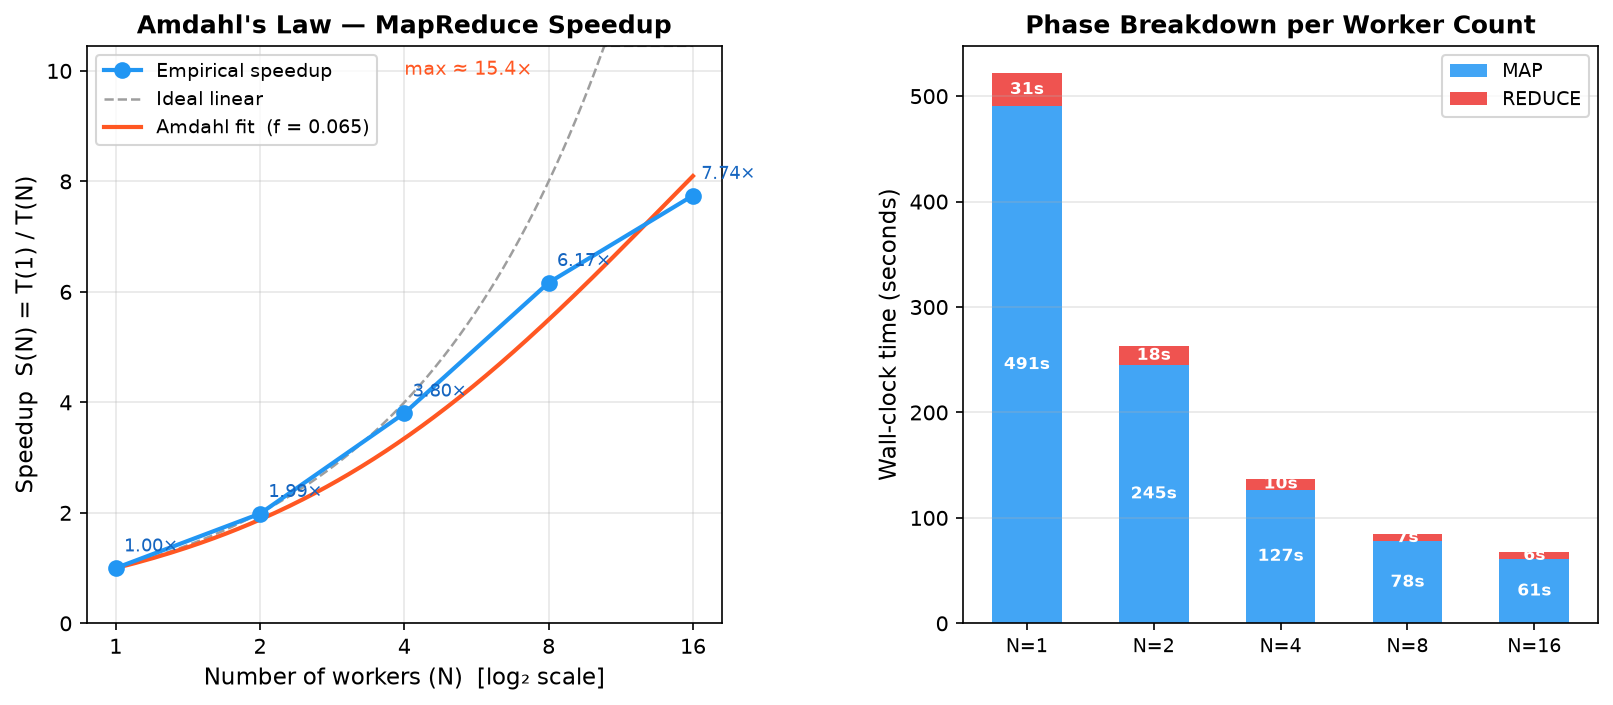
\includegraphics[width=\textwidth]{amdahl_cluster.png}
\caption{Cluster Amdahl's law. Left: measured speedup vs ideal-linear, with a
fitted serial fraction $f=0.065$ implying a theoretical ceiling of $\approx
15.4\times$. Right: per-worker-count wall-clock split into MAP (blue) and REDUCE
(red), showing MAP dominates and shrinks near-linearly with $N$.}
\label{fig:cluster}
\end{figure}

The measured curve tracks the Amdahl fit closely: $1.99\times,\,3.80\times,\,
6.17\times,\,7.74\times$ at $N=2,4,8,16$. The fitted $f=0.065$ is small because
the workload is embarrassingly parallel in its MAP phase; the residual serial
part is the \code{MAP$\to$REDUCE} barrier, the portion of shuffle that cannot
overlap, master bootstrap, and final output collection. As $N$ approaches the
number of splits, the marginal gain shrinks (there is simply less MAP work to
hand out), which is exactly why the empirical curve bends below ideal-linear at
$N=16$.

\paragraph{Why the sweep stops at 16 and not at 100.} The lab platform has
\emph{100+} machines, and the engine can address all of them: Day~1 deploys the
load-average server to the full pool (\S\ref{sec:cpuload}) and the Main can hand
tasks to as many workers as we register. The Amdahl study is nonetheless capped
at $N=16$ on purpose, because it is a \emph{strong-scaling} experiment: the rule
from the brief is that \textbf{the dataset must stay identical at every point},
and our fixed benchmark is cut into \textbf{16 splits} (one MAP task each). With
16 MAP tasks, any worker beyond the 16th simply has no MAP work to claim and
sits idle, so $N>16$ \emph{cannot} raise the MAP speedup, it only adds
scheduling and barrier overhead and would bend the curve further below ideal.
The two numbers therefore describe different things and are consistent:
\textbf{100} is the \emph{platform capacity} (and what weak scaling, growing the
data and the workers together, would exploit), whereas \textbf{16} is the
largest worker count at which \emph{this fixed dataset} still yields meaningful
parallelism. Pushing $N$ to 100 here would just plot a flat line past 16, which
is why we report the strong-scaling curve only where it is informative.

\subsection{Single-machine sweep (reproducible by one person)}

For reproducibility without a cluster, \code{tests/run\_all.py} runs the same
methodology with several worker processes on one box (8 splits, 8 reducers,
fixed synthetic dataset):

\begin{table}[H]
\centering
\small
\renewcommand{\arraystretch}{1.2}
\begin{tabular}{@{}rrr@{}}
\toprule
$N$ & $t_{\text{total}}$ (s) & speedup\\
\midrule
1 & 1.584 & 1.00$\times$\\
2 & 1.006 & 1.57$\times$\\
4 & 0.826 & \textbf{1.92$\times$}\\
\bottomrule
\end{tabular}
\caption{Single-machine sweep.}
\end{table}

\begin{figure}[H]
\centering
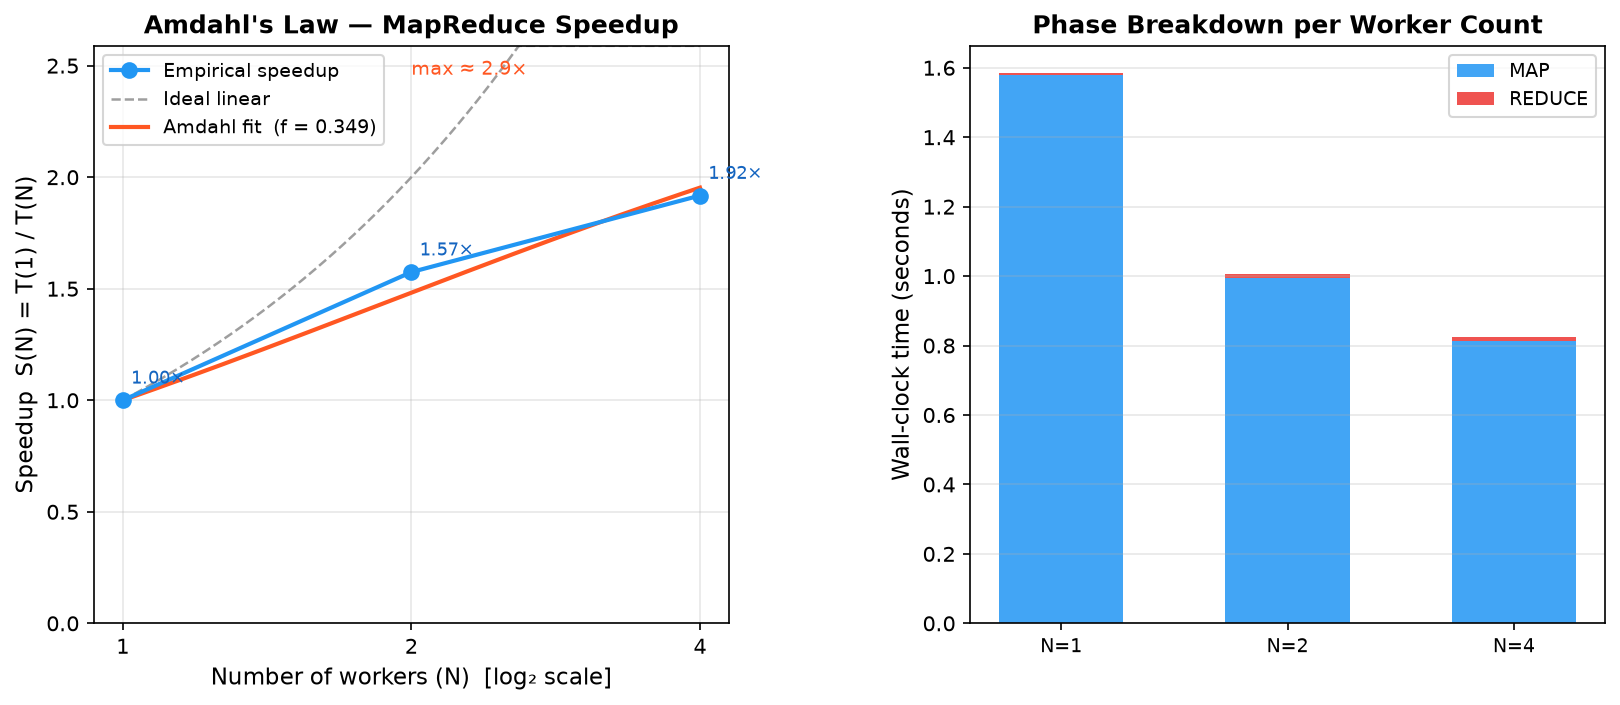
\includegraphics[width=\textwidth]{amdahl_speedup.png}
\caption{Single-machine Amdahl's law. The fitted $f=0.349$ is \emph{larger}
than on the cluster: co-located worker processes share one machine's memory
bandwidth and disk, inflating the serial fraction and capping the ceiling near
$2.9\times$. This contrast between the two figures is itself the lesson, Amdahl's
$f$ is a property of the \emph{whole system}, not just the algorithm.}
\label{fig:solo}
\end{figure}

\subsection{Interpretation}

The two figures together tell the full story: on dedicated hardware the engine
scales close to linear ($f=0.065$, $7.74\times$ at $N=16$); crammed onto a single
shared machine it hits a wall near $3\times$ ($f=0.349$). The per-build
optimisations (\S\ref{sec:opt-scaling}) then lower absolute time while
\emph{raising} the serial fraction $f$ --- and on-demand ingestion
(\S\ref{sec:opt-ondemand}) even escapes the bound superlinearly --- so $f$ is a
property of the \emph{whole system} (algorithm, I/O path, and hardware), exactly
as Amdahl predicts, demonstrated empirically and reproducibly.

% =============================================================================
\section{Fault tolerance}\label{sec:ft}
% =============================================================================

V1 had a fatal flaw discovered by stress-testing: a \emph{single} dead worker
froze the whole job forever (the completion counter never reached the total, so
the Main hung and had to be killed by hand). V2 adds five mechanisms from the
paper~(\S3.1–3.6), \emph{without changing the happy path}.

\subsection{1. Failure detection (heartbeat + lease)}

Workers heartbeat every \code{HEARTBEAT\_INTERVAL = 2\,s}. The Main arms a
\code{recv()} lease of \code{LEASE\_TIMEOUT = 60\,s} on each connection. Two
distinct failures are caught:
\begin{itemize}
\item \textbf{Process/host crash}, the TCP socket closes, \code{recv()} returns
empty \emph{immediately}, regardless of the lease.
\item \textbf{Network partition / hang}, no bytes arrive; the lease expires and
the worker is declared dead.
\end{itemize}
The lease (60\,s) is deliberately well above a single real-split MAP
($\sim$30\,s of GIL-bound pure-Python compute, during which the background
heartbeat thread cannot grab the GIL). This avoids wrongly killing a
\emph{busy but healthy} worker, while a genuine crash is still detected
instantly via socket close.

\subsection{2. Task reassignment (re-execution rules)}

When a worker dies, \code{\_reclaim()} applies the paper's rules exactly:

\begin{table}[H]
\centering
\small
\renewcommand{\arraystretch}{1.25}
\begin{tabularx}{\textwidth}{@{}lX@{}}
\toprule
\textbf{State on dead worker} & \textbf{Action}\\
\midrule
in-progress MAP or REDUCE & re-queue the task\\
\textbf{completed MAP} & \textbf{re-run}, its \code{/tmp} output died with the machine\\
\textbf{completed REDUCE} & \textbf{keep}, output was committed atomically to NFS\\
MAP source dies \emph{during} REDUCE & revert to MAP phase, re-run lost maps, re-queue \emph{all} reduces\\
\bottomrule
\end{tabularx}
\end{table}

The last rule is heavy but correct: if a machine that produced a partition dies
after the barrier, reducers can no longer fetch from it, so the Main rebuilds the
shuffle sources by recomputing the lost maps and redoing the reduces (safe
because reduce output is idempotent and atomic).

\subsection{3. Atomic output commit (exactly-once)}

A reducer writes \code{part-j.<pid>.tmp} and then \code{os.replace()}s it into
\code{part-j.txt}. Since \code{os.replace} is an atomic rename on the same
filesystem, a reducer that crashes mid-write \emph{never} leaves a half-written
file, and a re-executed reducer cleanly overwrites the previous attempt. This is
what makes ``keep completed REDUCE'' safe.

\subsection{4. Straggler backup tasks (\S3.6)}

When the MAP queue is empty but tasks are still in flight, an idle worker is
handed a \emph{duplicate} of the slowest in-flight split (older than
\code{STRAGGLER\_THRESHOLD = 90\,s}). Whichever copy finishes first wins; the
loser's late \code{TASK\_FINISHED} is recognised as stale (the task is already
\code{completed}) and discarded.

\subsection{5. Master recovery (designed, not implemented)}

The space-time design (Fig.~\ref{fig:ft}) includes Main checkpointing to NFS and
resuming from the last barrier on restart. We state this plainly in the self-assessment:
this is \emph{specified in the protocol but not implemented in code}, worker
fault tolerance is fully working; master recovery is future work.

\begin{figure}[H]
\centering
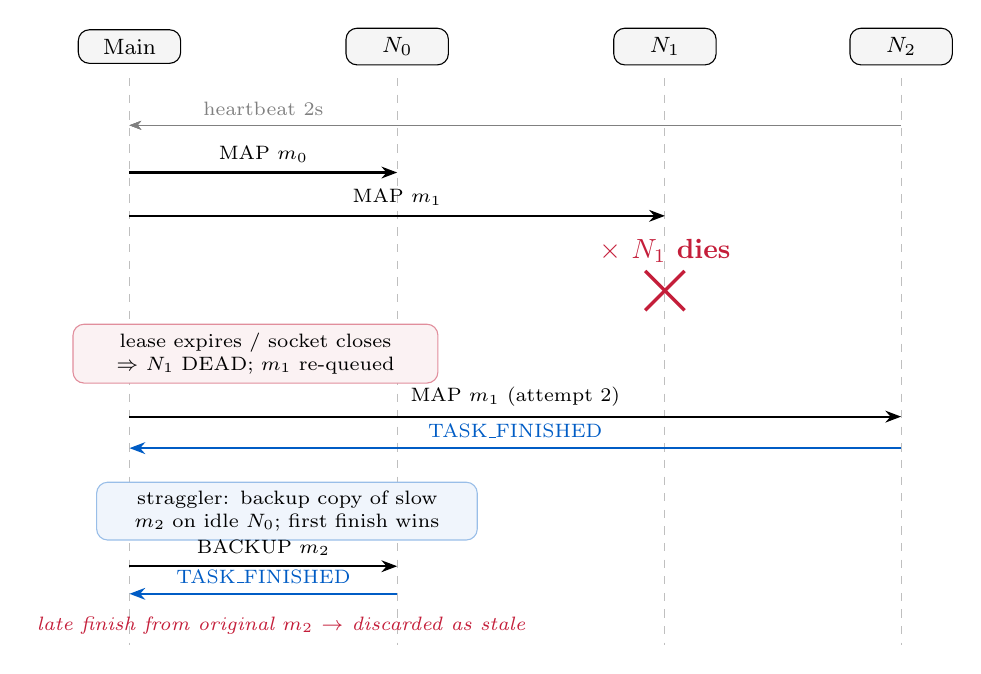
\begin{tikzpicture}[font=\footnotesize]
\def\xM{0} \def\xA{3.4} \def\xB{6.8} \def\xC{9.8}
\foreach \x/\name in {\xM/{Main}, \xA/{$N_0$}, \xB/{$N_1$}, \xC/{$N_2$}} {
  \node[draw,fill=gray!8,rounded corners,minimum width=1.3cm] at (\x,0) {\name};
  \draw[gray!50,dashed] (\x,-0.4) -- (\x,-7.6);
}
\tikzset{msg/.style={-{Stealth[length=2mm]},thick}}
\tikzset{ret/.style={-{Stealth[length=2mm]},thick,accentblue}}
\tikzset{hb/.style={-{Stealth[length=1.5mm]},thin,gray}}
% heartbeats
\draw[hb] (\xA,-1.0) -- node[above,sloped,font=\scriptsize,gray]{heartbeat 2s} (\xM,-1.0);
\draw[hb] (\xB,-1.0) -- (\xM,-1.0);
\draw[hb] (\xC,-1.0) -- (\xM,-1.0);
% assign maps
\draw[msg] (\xM,-1.6) -- node[above,sloped,font=\scriptsize]{MAP $m_0$} (\xA,-1.6);
\draw[msg] (\xM,-2.15) -- node[above,sloped,font=\scriptsize]{MAP $m_1$} (\xB,-2.15);
% N1 dies
\node[accent,font=\bfseries] at (\xB,-2.6) {$\times$ $N_1$ dies};
\draw[accent,very thick] (\xB-0.25,-2.85) -- (\xB+0.25,-3.35);
\draw[accent,very thick] (\xB+0.25,-2.85) -- (\xB-0.25,-3.35);
% lease expiry note
\node[draw=accent!50,fill=accent!6,rounded corners,font=\scriptsize,text width=4.4cm,align=center] at (\xM+1.6,-3.9) {lease expires / socket closes\\ $\Rightarrow$ $N_1$ DEAD; $m_1$ re-queued};
% reassign to N2
\draw[msg] (\xM,-4.7) -- node[above,sloped,font=\scriptsize]{MAP $m_1$ (attempt 2)} (\xC,-4.7);
\draw[ret] (\xC,-5.1) -- node[above,sloped,font=\scriptsize]{TASK\_FINISHED} (\xM,-5.1);
% backup task
\node[draw=accentblue!40,fill=accentblue!6,rounded corners,font=\scriptsize,text width=4.6cm,align=center] at (\xM+2.0,-5.9) {straggler: backup copy of slow $m_2$ on idle $N_0$; first finish wins};
\draw[msg] (\xM,-6.6) -- node[above,sloped,font=\scriptsize]{BACKUP $m_2$} (\xA,-6.6);
\draw[ret] (\xA,-6.95) -- node[above,sloped,font=\scriptsize]{TASK\_FINISHED} (\xM,-6.95);
\node[anchor=west,accent,font=\scriptsize\itshape] at (-1.3,-7.35) {late finish from original $m_2$ $\to$ discarded as stale};
\end{tikzpicture}
\caption{Fault-tolerance protocol (V2), simplified. Heartbeats feed a lease-based
detector; a dead worker's in-progress and completed-MAP tasks are re-executed;
stragglers get backup copies. Full source:
\code{doc/fault\_tolerance/fault\_tolerance.seqdiag.txt}.}
\label{fig:ft}
\end{figure}

\subsection{Demonstrating it}

\code{src/deploy/fault\_tolerance\_demo.sh} kills $N$ worker processes mid-job;
the Main logs the detection and reassignment, and the job still completes with a
correct result. The single-machine \code{run\_all.py} automates this: it kills a
worker mid-run and asserts the final output still matches the reference.

% =============================================================================
\section{Validation}\label{sec:validate}
% =============================================================================

\code{src/mapreduce/validate.py} is the correctness oracle. It \emph{imports the
worker's own \code{\_map\_emit}} so the reference computation cannot drift from
the distributed one, recomputes the chosen analysis on a single machine over the
same splits, and compares against the aggregated \code{part-*.txt}:

\begin{enumerate}
\item number of distinct keys (reference vs distributed),
\item sum of all counts,
\item per-key equality (every key has the same count on both sides).
\end{enumerate}

It prints the top-$N$ and exits \code{0}=PASS / \code{1}=FAIL / \code{2}=error.
This is the ``run a single-machine word count on the same dataset and confirm
identical counts'' check from the brief, generalised to all four jobs.

% =============================================================================
\section{Kafka Streams comparison}\label{sec:kafka}
% =============================================================================

To contrast our \emph{batch} engine with a \emph{streaming} one, we orchestrate
the official Apache Kafka (4.x) in \textbf{KRaft mode}, \textbf{no Docker, no
root, no ZooKeeper}, all state under \code{/tmp} so NFS is untouched. We did not
write a stream processor; we drive Apache's prebuilt \code{WordCountDemo} with
four small Bash scripts.

\begin{table}[H]
\centering
\small
\renewcommand{\arraystretch}{1.2}
\begin{tabularx}{\textwidth}{@{}lX@{}}
\toprule
\textbf{Script} & \textbf{Role}\\
\midrule
\code{deploy\_kafka.sh} & download + start a single-node KRaft broker on \code{/tmp}\\
\code{run\_wordcount.sh} & create topics, reset app state, run \code{WordCountDemo}, feed input, print top-$N$\\
\code{commoncrawl\_source.sh} & stream a Common Crawl split \emph{directly} into the input topic (no file)\\
\code{clean\_kafka.sh} & stop the app + broker and wipe data (\code{-a} for a full wipe)\\
\bottomrule
\end{tabularx}
\end{table}

\paragraph{Why an \code{awk} post-step.} The output topic is a \emph{compacted
changelog}: each word is re-emitted with a growing count
(\code{the$\to$1, the$\to$2, \dots}). We keep the \emph{last} value per key, then
sort:
\begin{lstlisting}[language=bash]
awk -F'\t' 'NF==2 {last[$1]=$2} END {for (k in last) print last[k]"\t"k}' \
    | sort -rn | head -n "$TOP_N"
\end{lstlisting}

\paragraph{Direct Common Crawl $\to$ Kafka source.}
\code{commoncrawl\_source.sh} is a single shell pipeline,
\code{curl | gunzip | grep -v headers | head | kafka-console-producer}, that
resolves a split from \code{wet.paths.gz} and streams it into
\code{streams-plaintext-input} with \emph{zero} intermediate files. It is the
streaming analogue of our native \code{-{}-direct-read}: the batch side streams
Amazon $\to$ RAM, the stream side streams Amazon $\to$ Kafka topic.

\paragraph{Result.} The top words (\code{the, to, of, and, a, \dots}) are
\emph{identical} to our batch engine's output. The difference is purely
operational: Kafka keeps the result live and updates it forever; our job emits
one final answer and exits.

% =============================================================================
\section{Comparison: our system vs Hadoop vs Kafka Streams}\label{sec:compare}
% =============================================================================

\textbf{Batch vs stream in one line.} Batch (our system, Hadoop) reads bounded
input, runs to completion, emits a final result once. Stream (Kafka Streams)
reads unbounded input and produces an incremental result that never ``finishes''.

\begin{table}[H]
\centering
\small
\renewcommand{\arraystretch}{1.3}
\begin{tabularx}{\textwidth}{@{}lXXX@{}}
\toprule
\textbf{Dimension} & \textbf{Our system} & \textbf{Hadoop MapReduce} & \textbf{Kafka Streams}\\
\midrule
Model & Batch & Batch & Stream (continuous)\\
Language & Python (+ Bash) & Java & Java/Scala\\
Storage & NFS + local \code{/tmp}, manual remote read & HDFS (locality, replication) & Kafka topics (log)\\
Scheduling & our Main, 1 task/worker pull & YARN, speculative exec & broker-side assignment\\
Fault tolerance & heartbeat + re-exec + atomic writes & re-exec + speculative + HDFS replication & changelog + state-store restore\\
Output & final \code{part-*.txt} once & final files in HDFS once & live, updated changelog topic\\
Setup difficulty & low (scripts, no deps) & high (cluster, HDFS, YARN) & medium (download broker, no root)\\
Result on same data & identical (validated) & identical & identical \emph{final} counts\\
\bottomrule
\end{tabularx}
\caption{Three paradigms on the same word-count task.}
\end{table}

\textbf{What our deliberately-simplified system lacks vs Hadoop:} no HDFS (no
data-locality scheduling, block replication, or rack awareness), no YARN
multi-tenancy, no combiner/partitioner plugin API, no speculative execution at
Hadoop's level, no secure RPC, no job-history server. We re-implemented only the
\emph{core ideas}, map/shuffle/reduce, hash partitioning, local intermediates +
remote read, re-execution, backup tasks, precisely to understand them from the
inside.

% =============================================================================
\section{Pain points: what broke and why}\label{sec:pain}
% =============================================================================

\begin{itemize}
\item \textbf{NFS overload.} Reading hundreds of splits from the internal NFS at
once made the shared server crawl. \emph{Fix:} intermediates to local \code{/tmp};
direct streaming of Common Crawl from Amazon, removing the NFS read path.
\item \textbf{SSH fan-in / IDS.} Many parallel \code{ssh} connections per host
risked tripping \code{fail2ban}. \emph{Fix:} \code{ControlMaster=auto}
multiplexing (one real TCP connection per host) plus a \code{max\_ssh} cap.
\item \textbf{A single dead worker froze the whole job (V1).} No failure
detection meant the Main hung forever. \emph{Fix:} the V2 fault-tolerance
protocol.
\item \textbf{Partial/corrupt reduce output on a mid-write crash.} \emph{Fix:}
atomic \code{.tmp} + \code{os.replace()} commit.
\item \textbf{Busy worker wrongly declared dead.} An early, short lease killed
healthy workers mid-MAP (the GIL starves the heartbeat thread during a 30\,s
compute). \emph{Fix:} raise the lease to 60\,s, well above one MAP, while still
catching real crashes instantly via socket close.
\item \textbf{Scaling wall.} We expected near-linear scaling; measurement showed
a hard ceiling, a concrete lesson in Amdahl's law.
\item \textbf{Campus Wi-Fi / WSL2 flakiness.} Intermittent SSH drops; mitigated
with timeouts, \code{ServerAliveInterval}, \code{BatchMode}, and idempotent
deploy/clean scripts.
\end{itemize}

% =============================================================================
\section{Deployment and reproducibility}\label{sec:deploy}
% =============================================================================

\subsection{Cluster deployment}

\begin{lstlisting}[language=bash]
# Deploy master + N workers, run a job on the cluster
bash src/deploy/deploy_commoncrawl.sh -w 8 -r 8 -s 20 -j wordcount
bash src/deploy/deploy_commoncrawl.sh -w 8 -r 8 -s 20 -j bigram

# Inject a fault mid-job (second terminal) and watch the master recover
bash src/deploy/fault_tolerance_demo.sh -n 1

# Validate the distributed output against a single-machine reference
python3 src/mapreduce/validate.py -i <input> -o <output> -j wordcount

# Tear everything down (idempotent; -d also deletes NFS output)
bash src/deploy/kill_commoncrawl.sh -d
\end{lstlisting}

\code{deploy\_commoncrawl.sh} fetches live machines, SCPs the engine to NFS,
downloads only the missing splits, starts the Main, then starts $N$ workers in
parallel and streams the Main log live until the job finishes.

\subsection{One-command single-machine reproduction}

No cluster, no teammates:
\begin{lstlisting}[language=bash]
python3 tests/run_all.py            # correctness (4 jobs) + fault tolerance + Amdahl sweep
python3 tests/run_all.py --quick    # correctness + FT only
\end{lstlisting}
This spins up a real Main and several real workers on \code{localhost}, checks
all four analyses against the reference, kills a worker to prove fault tolerance,
and regenerates the Amdahl figure, exit code \code{0} only if everything passes.

\subsection{Kafka demo}

\begin{lstlisting}[language=bash]
bash src/kafka/deploy_kafka.sh                      # start a KRaft broker on /tmp
bash src/kafka/run_wordcount.sh --crawl CC-MAIN-2024-10   # stream CC -> topic -> top-N
bash src/kafka/clean_kafka.sh -a                    # full teardown
\end{lstlisting}

% =============================================================================
\section{Implementation map: concept to code}\label{sec:implmap}
% =============================================================================

Every concept, optimisation and mechanism discussed in this report is backed by
a specific file (and, where useful, a function) in the repository. The table
below is the single index a reader can use to jump from an idea to the code that
implements it.

\begin{table}[H]
\centering
\small
\renewcommand{\arraystretch}{1.25}
\begin{tabularx}{\textwidth}{@{}X l@{}}
\toprule
\textbf{Concept / optimisation} & \textbf{File\,:\,function}\\
\midrule
Live-machine discovery (school API, filter free hosts) & \code{src/deploy/get\_machines.py}\\
CPU-load TCP server / parallel client (Day 1) & \code{src/server/server.py}, \code{src/client/client.py}\\
Coordinator: task queues, MAP$\to$REDUCE barrier, detector & \code{src/mapreduce/master.py}\\
Worker process (MAP and REDUCE execution) & \code{src/mapreduce/worker.py}\\
MAP tokenise + per-job keying (4 analyses) & \code{worker.py\,:\,\_map\_emit}\\
\textbf{Opt 1}: combine + bytes-regex + vectorised CRC32 & \code{worker.py\,:\,\_execute\_map}\\
Hash partitioning \code{crc32(k)\,\%\,R} & \code{worker.py\,:\,\_execute\_map}\\
\textbf{Opt 2}: parallel SSH shuffle + ControlMaster mux & \code{worker.py\,:\,\_execute\_reduce}\\
Atomic exactly-once output (\code{.tmp} + \code{os.replace}) & \code{worker.py\,:\,\_execute\_reduce}\\
Direct S3 streaming read (\code{-{}-direct-read}) & \code{worker.py\,:\,\_stream\_crawl\_bytes}\\
WET/WARC header stripping & \code{worker.py\,:\,\_strip\_wet\_headers}\\
Common Crawl prefetch to spill dir & \code{src/mapreduce/download\_commoncrawl.py}\\
Failure detection (heartbeat + lease) & \code{src/mapreduce/master.py}\\
Re-execution + backup tasks (stragglers) & \code{master.py\,:\,\_reclaim}, \code{\_pick\_backup\_split}\\
Correctness validation (sequential reference) & \code{src/mapreduce/validate.py}\\
Scratch-disk discovery (avoid \code{tmpfs}) & \code{src/benchmarks/find\_scratch.sh}\\
SSH parallelism sweep (tune \code{max\_ssh}) & \code{src/benchmarks/ssh\_parallelism\_sweep.py}\\
Amdahl cluster sweep + figures & \code{src/benchmarks/amdahl\_bench.py}, \code{plot\_amdahl.py}\\
Deployment (1 SCP + $N$ SSH) & \code{src/deploy/deploy\_commoncrawl.sh}\\
Kafka Streams comparison (KRaft, no Docker) & \code{src/kafka/run\_wordcount.sh}\\
One-command single-machine reproduction & \code{tests/run\_all.py}\\
\bottomrule
\end{tabularx}
\caption{From idea to implementation: where each part of the system lives.}
\label{tab:implmap}
\end{table}

% =============================================================================
\section{Anticipated questions and design rationale (defense Q\&A)}\label{sec:qa}
% =============================================================================

This project invites a particular kind of probing question: ``why did
this not break?'', ``what happens at scale?'', ``prove it''. Rather than leave
those answers to the oral defense, we make the reasoning behind each choice
explicit here, anchored in the actual code.

\subsection{Memory: why we never saturated RAM, and how we would guarantee it}
\label{sec:qa-mem}

\textbf{Q: A reducer fetches \code{partition\_j.txt} from every map worker and
sums it. Loading whole partitions into memory should blow up, why didn't you
see RAM saturation?}

\medskip\noindent The answer has two halves: \emph{why it held in
practice}, and \emph{how we would make it hold at any scale}.

\paragraph{Why it held: the map-side combiner.} The decisive reason is that MAP
\emph{pre-aggregates} before writing (\S\ref{sec:opt}). In
\code{worker.py}, the MAP phase makes one pass that folds \emph{all} occurrences
into a dict, so each \code{partition\_j.txt} contains \textbf{one line per unique
key} (\code{the\textbackslash t79745}), not 79{,}745 separate
\code{the\textbackslash t1} lines. On our real split this collapses the
intermediate data from $\approx$\textbf{6.6\,M} token emissions to
$\approx$\textbf{435\,k} distinct-key lines, more than a 10$\times$ reduction,
\emph{before anything is shuffled}. Two further factors compound it:
\begin{itemize}[leftmargin=1.4em]
  \item \textbf{Hash partitioning} \code{crc32(k)\,\%\,R} sends each reducer only
  $1/R$ of the key space (with $R=8$, $\approx$54\,k keys per reducer);
  \item the reducer's live state is just a \code{dict[str,int]} of short keys,
  a few megabytes, trivial against the machines' multi-GB RAM.
\end{itemize}
So $16$ splits $\times$ 435\,k keys, pre-aggregated and split $8$ ways, is a few
MB per reducer: nowhere near saturation.

\paragraph{The real inefficiency: an in-memory hash-merge, not an external
sort-merge.} Beyond raw RAM there is an \emph{algorithmic} objection worth naming
explicitly, because it is the sharpest critique of the reduce path. For each of
the $M$ map sources the reducer calls \code{readlines()} and \code{extend}s every
line into a single \code{all\_raw\_lines} list, and only \emph{then} folds that
list into the \code{final\_counts} dict. So at peak it holds \emph{two} full
copies of its shuffle input --- the raw-line list \emph{and} the growing hash map
--- and performs the merge as one big \textbf{unsorted, in-memory hash
aggregation over all $M$ partitions at once}. This departs from the canonical
MapReduce reducer in three costly ways:
\begin{itemize}[leftmargin=1.4em]
  \item \textbf{Double materialisation.} Buffering into \code{all\_raw\_lines}
  before aggregating is pure overhead: $O(\text{all incoming lines})$ memory plus
  a large short-lived list for the garbage collector to churn. Folding each line
  \emph{as it streams in} would both halve peak memory and let the merge overlap
  the shuffle I/O.
  \item \textbf{No sorted runs $\Rightarrow$ no streaming $k$-way merge.} Because
  MAP writes each partition in \emph{hash} order rather than \emph{sorted} order,
  the reducer cannot do the textbook external merge of $M$ pre-sorted runs ---
  which touches only one line per source at a time, needs $O(\#\text{sources})$
  memory, and is sequential and cache-friendly. Instead it pays for a full hash
  table over the entire partition, with the random-access and rehash costs that
  implies. This is precisely the ``a ton of in-memory merging'' inefficiency: the
  work that Hadoop/Spark push into a disk-backed sort-merge, we currently do
  eagerly in one RAM-resident dict.
  \item \textbf{Sorted output is a \emph{partial} by-product.} We currently sort
  the final counts by \emph{count} (descending) before writing, whereas an
  external merge sorts by \emph{key}; the two orders differ, so the ranking would
  not come entirely for free. A key-sorted merge would still eliminate the
  separate hash table, and re-ranking the already-reduced keys by count is then a
  cheap final pass over the \emph{distinct} keys only (a few $\times10^4$ per
  reducer), not over the raw shuffle input.
\end{itemize}
It never bit us at $16$ splits --- the combiner keeps the working set at a few MB
(above) --- but the observation is exactly right: this is the part of the design
that would not survive a TB-scale partition, and the fix is the external
sort-merge listed last below.

\paragraph{How we guarantee it at any scale.} Four levers, in order of effort:
\begin{enumerate}[leftmargin=1.6em]
  \item \textbf{Stream the shuffle into the counter} instead of buffering it,
  fold each line as it arrives so memory becomes $O(\text{distinct keys in this
  reducer})$, not $O(\text{all lines})$:
\begin{lstlisting}[language=python]
for line in proc.stdout:          # iterate, do NOT readlines()
    k, _, v = line.partition("\t")
    counts[k] = counts.get(k, 0) + int(v)
\end{lstlisting}
  \item \textbf{Keep the map-side combiner} (already our biggest win);
  \item \textbf{Raise $R$}, more reducers shrink each reducer's key space
  linearly;
  \item \textbf{External sort-merge / spill to disk}, the real guarantee: have
  each MAP write its partition \emph{sorted by key}, then the reducer does a
  streaming $k$-way merge holding only \emph{one line per source} at a time, so
  memory is $O(\#\text{sources})$, independent of data size. This is exactly what
  Hadoop and Spark do, and it is the textbook answer to ``what if even the
  per-reducer dict does not fit?''.
\end{enumerate}

\subsection{Storage and shuffle}

\paragraph{Q: When a worker writes to its \code{\$HOME}, where does that land?}
On the \textbf{NFS}, not local disk, which is precisely why MAP intermediates go
to \code{/tmp} (local disk), as in Figure~1 of the paper: writing intermediates
to NFS would saturate the shared server (\S\ref{sec:arch}).

\paragraph{Q: \code{/tmp} can be a RAM-backed \code{tmpfs}: isn't that a trap?}
Yes; on some nodes \code{/tmp} is a small \code{tmpfs} that would fill under
hundreds of concurrent splits. We therefore probe for a large scratch partition
(\code{find\_scratch.sh}) and point \code{--local-map-dir} there, falling back to
\code{/tmp} only when no better disk exists.

\paragraph{Q: How does a reducer read intermediates written locally on the maps?}
By \textbf{remote read}: the Main hands the reducer the \{host, map\_dir\} of
every map; the reducer runs \code{ssh host cat partition\_j.txt} against \emph{all}
maps \textbf{in parallel} and sums. The bytes never transit the Main
(\S\ref{sec:protocol}).

\paragraph{Q: Wouldn't a raw TCP transfer have been faster than \code{ssh cat}?}
On the wire, marginally yes; for this project, no --- and the numbers say the gap
is not worth chasing. A raw-TCP shuffle avoids the SSH handshake, the per-fetch
crypto, and forking a remote shell$+$\code{cat}. But three things make it the
wrong trade here:
\begin{itemize}[leftmargin=1.4em]
  \item \textbf{We already amortised SSH's cost.} \code{ControlMaster=auto}
  collapses every fetch to \emph{one} real TCP connection per host, reused across
  reducers (\code{ControlPersist}), and the parallel \code{ThreadPoolExecutor}
  floors shuffle wall-time at \textbf{1--5\,s across all $N$}
  (\S\ref{sec:opt-scaling}). Shuffle is only $\approx$3--5\% of the wall, so even
  a \emph{free} transport would shave a few percent at most --- Amdahl again.
  \item \textbf{SSH gives us auth, encryption, and zero deployment for free.} Raw
  TCP means running our \emph{own} data-serving daemon on every worker: an extra
  process to deploy, supervise and tear down, plus its own framing and
  connection management. We assume the university cluster is a \emph{trusted}
  network, so the encryption/authentication SSH provides is not something we
  strictly need here; but on any untrusted network an unauthenticated data port
  would be a real exposure, and SSH gives that protection for free with no extra
  work on our side.
  \item \textbf{\code{ssh cat} is trivially correct.} A hand-rolled TCP protocol
  needs framing, partial-read handling, backpressure and error recovery --- code
  that can only lose against a one-line \code{cat} at our scale.
\end{itemize}
Raw TCP becomes the right answer only when shuffle actually dominates the wall
(hundreds of workers, TB-scale partitions), and even then the bigger win is
\emph{pushing} partitions from mappers as they finish so transfer overlaps
compute, rather than pulling them afterwards --- both are listed as future work
(\S\ref{sec:opt}).

\paragraph{Q: How do you decide which node owns which key at reduce time?}
We assign each key with \code{crc32(key)\,\%\,n\_reducers}. It is deterministic,
so all occurrences of a key land on the same reducer, \textbf{as long as the
reducer count stays constant} for the job. Change it mid-job and counts shatter
across reducers.

\subsection{Correctness and output}

\paragraph{Q: Are your results correct, and how do you prove it?}
\code{validate.py} recomputes each analysis on a \emph{single} machine,
sequentially, and compares key-by-key against the distributed output, and it
\textbf{reuses the worker's own tokeniser} so we never compare two different
logics (\S\ref{sec:validate}). We obtain an exact PASS.

\paragraph{Q: Are your writes atomic?}
Yes: write to a \code{.tmp} on the same directory, then \code{os.replace()}
(atomic rename). A reducer that dies mid-write never leaves a half-written
\code{part-*.txt}, and a re-executed reducer cleanly overwrites, exactly-once
output (\S\ref{sec:ft}).

\subsection{Fault tolerance}

\paragraph{Q: How do you detect that a worker died?}
Heartbeats every 2\,s plus a lease on the Main. A killed process closes its TCP
socket (immediate detection); a network partition simply lets the lease expire
(\S\ref{sec:ft}).

\paragraph{Q: Why a 60\,s lease and not less?}
A real MAP spends $\approx$30\,s in GIL-bound pure-Python compute during which no
heartbeat can be sent; too short a lease would kill \emph{healthy} workers. A true
crash is caught instantly by the TCP close, so 60\,s does not slow real detection.

\paragraph{Q: A completed MAP on a machine that then dies: is the data lost?}
Yes, its partitions were on that node's local \code{/tmp}, so we \textbf{re-run}
the map. A completed \emph{reduce}, by contrast, is kept: its output is already on
NFS, written atomically (\S\ref{sec:ft}).

\paragraph{Q: Do you handle slow machines (stragglers)?}
Yes, the paper's backup tasks (\S3.6): past a threshold, a copy of the slow task
is given to an idle worker and the first to finish wins; the late duplicate is
discarded as stale.

\paragraph{Q: And if the Main dies?}
That is our stated limit: the Main is a single point of failure. Checkpoint/
recovery (\S3.2 of the paper) is \emph{designed} (sequence diagram) but
\emph{not implemented}, and we say so plainly (\S\ref{sec:pain}).

\subsection{Performance and scaling}

\paragraph{Q: What is the bottleneck, and can you prove it?}
The MAP \code{t\_compute}, \textbf{>85\%} of worker time, \emph{measured} from
the per-phase \code{WORKER\_TIMING} log lines, not assumed. That is exactly what
we targeted with the combiner + byte-level regex optimisation
(\S\ref{sec:opt},~\S\ref{sec:perf}).

\paragraph{Q: Do you have a reference point for Amdahl, and the same dataset
everywhere?} Yes: $N=1\Rightarrow S=1$, the \emph{same dataset at every point};
we only interpolate on a single machine and \emph{measure} from two nodes up
(\S\ref{sec:amdahl}).

\paragraph{Q: Why does the sweep stop at 16 workers when you talk about 100
machines?} Because it is a \emph{strong-scaling} study on a fixed 16-split
dataset: beyond 16 workers there is no MAP work left to hand out. ``100'' is the
\emph{platform capacity}; ``16'' is the largest worker count at which this fixed
dataset still yields parallelism (full argument in \S\ref{sec:amdahl}).

\subsection{Deployment and ecosystem}

\paragraph{Q: One SCP then $N$ SSH: why better than $N$ SCP?}
\code{\$HOME} is on NFS, \emph{shared} by every machine: copy the engine
\textbf{once} to NFS (1 SCP), then launch the servers over SSH ($N$ SSH). Since
NFS is visible everywhere, copying $N$ times is pointless (\S\ref{sec:deploy}).

\paragraph{Q: How do you find live machines?}
Via the school API (\code{tp.telecom-paris.fr}): we parse the raw JSON, filter for
\emph{live} and \emph{free} hosts sorted by load (\code{get\_machines.py}), and
keep a verified, SSH-reachable list for the demo so we never depend on the live
API mid-presentation (\S\ref{sec:cpuload}).

\paragraph{Q: Batch vs stream: did you actually run Kafka Streams?}
Yes, a Kafka broker in KRaft mode (no Docker/root), \code{WordCountDemo} over a
real Common Crawl split. The final counts are \textbf{identical} to ours; the
difference is that Kafka updates continuously via a changelog, whereas we produce
one final result and stop (\S\ref{sec:kafka},~\S\ref{sec:compare}).

\paragraph{Q: What is missing versus Hadoop?}
HDFS (replication, data locality), YARN (multi-tenant scheduling), a generic
combiner/partitioner API, secured RPC, and a job-history server. We deliberately
built the \emph{conceptual core} to understand it, not a full Hadoop
(\S\ref{sec:compare}).

% =============================================================================
\section{Conclusion}\label{sec:conclusion}
% =============================================================================

We built a complete distributed MapReduce engine from first principles and took
it all the way from a naïve proof-of-concept to a fault-tolerant, instrumented,
multi-analysis system, validated against a single-machine oracle and benchmarked
on real hardware. The cluster scales to $7.74\times$ on 16 nodes with a measured
serial fraction of $0.065$; the single-machine reproduction confirms Amdahl's law
from the other direction, hitting a $\sim$3$\times$ wall under shared-resource
contention. Along the way we removed the NFS bottleneck with direct Amazon
streaming, hardened the protocol against worker death with heartbeats,
re-execution, atomic commits and backup tasks, generalised the engine to four
analyses behind one flag, and contrasted it with both Hadoop (batch) and a live
Kafka Streams pipeline (stream) computing the identical result.

\paragraph{Limitations.} Master recovery from checkpoint is designed but
not implemented; the reduce-phase-source-death recovery is correct but heavy
(it redoes all reduces); and large-scale runs (1000+ splits) are within the
engine's design but were exercised only into the tens of splits given lab time.
These are documented frankly in the accompanying self-assessment.

\begin{thebibliography}{9}
\bibitem{mapreduce} J.~Dean and S.~Ghemawat. \emph{MapReduce: Simplified Data
Processing on Large Clusters.} OSDI'04, San Francisco, 2004.
\bibitem{commoncrawl} Common Crawl Foundation. \emph{WET/WARC format and crawl
archives.} \url{https://commoncrawl.org}.
\bibitem{kafka} Apache Software Foundation. \emph{Apache Kafka, KRaft mode and
Kafka Streams WordCount example.} \url{https://kafka.apache.org}.
\end{thebibliography}

\end{document}
